\documentclass[titlepage]{report}
\usepackage[italian]{babel}
\usepackage[babel]{csquotes}
\usepackage[a4paper,left=2cm,bottom=2cm,right=2cm,top=2.5cm]{geometry}
\usepackage[utf8]{inputenc}
\usepackage[style=numeric-comp,useprefix,hyperref,backend=bibtex,natbib,sorting=none]{biblatex}
\usepackage{subcaption}
\usepackage{url}
\usepackage{graphicx} 			% pacchetto per inserire immagini
\usepackage{sidecap}			% pacchetto delle didascalie laterali
\usepackage{setspace}			% pacchetto per modificare interlinea
\usepackage{textcomp} 			% pacchetto per simboli unicode
\usepackage{xcolor}		% pacchetto colori per le celle delle tabelle
\usepackage{listings}
\usepackage{float}
\usepackage{nccmath}
\usepackage{hyperref}
\usepackage{xcolor}
\usepackage{parskip}
\usepackage{colortbl}
\usepackage{fancyhdr}
\usepackage[colorinlistoftodos,prependcaption,textsize=tiny]{todonotes} %using todo notes
\usepackage{xargs}   % personalizzazione dei comandi
%Frontespizio packages
\usepackage[nowrite,infront,standard,swapnames]{frontespizio}
%% Definizione nomi colori
\definecolor{codegreen}{rgb}{0,0.6,0}
\definecolor{codegray}{rgb}{0.5,0.5,0.5}
\definecolor{codepurple}{rgb}{0.58,0,0.82}
\definecolor{backcolour}{rgb}{0.98,0.98,0.95}


%% Revisione
\newcommandx{\condor}[2][1=]{\todo[linecolor=red,backgroundcolor=red!25,bordercolor=red,author=Luca,#1]{#2}}
\newcommandx{\simo}[2][1=]{\todo[linecolor=blue,backgroundcolor=blue!25,bordercolor=blue,author=Simone,#1]{#2}}
\newcommandx{\mike}[2][1=]{\todo[linecolor=green,backgroundcolor=green!25,bordercolor=green,author=Michele,#1]{#2}}

% Configurazioni per il pacchetto listings
\lstset{
  language=VHDL,
  basicstyle=\ttfamily\footnotesize,
  backgroundcolor=\color{backcolour},  
  keywordstyle=\color{blue}\bfseries,
  stringstyle=\color{orange},
  commentstyle=\color{green!60!black},
  numbers=left,
  numberstyle=\tiny,
  breakatwhitespace=false,         
  breaklines=true,                 
  captionpos=b,                    
  keepspaces=true,                 
  numbers=left,                    
  numbersep=5pt,                  
  showspaces=false,                
  showstringspaces=false,
  showtabs=false,                  
  tabsize=2,
  morekeywords={signal, process, if, elsif, else, std_logic}
}

\begin{document}  
% Per saltare una riga alla fine del paragrafo
\setlength{\parskip}{\baselineskip} 

\hypersetup{
	linkbordercolor={1 1 1},
}
\begin{frontespizio}
\end{frontespizio}
\tableofcontents
\newpage


\chapter*{Abstract}
\label{ch:intro}
\addcontentsline{toc}{chapter}{Abstract}


\chapter*{Architettura del sistema}
\label{ch:architettura}
\addcontentsline{toc}{chapter}{Architettura del sistema}

	\section*{FPGA Cyclone III}
	\label{sec:fpga}
	\addcontentsline{toc}{section}{FPGA Cyclone III}
		L'FPGA Cyclone III EP3C16F484C6, mostrata in figura \ref{fig:FPGA_cycloneIII}, è un dispositivo versatile e potente appartenente alla famiglia di FPGA prodotta da Intel, caratterizzato da specifiche e funzionalità avanzate che lo rendono adatto a diverse applicazioni.

		\begin{itemize}
			\item \textbf{Dimensioni}: L'FPGA è disponibile nella confezione 484-pin FineLine BGA, garantendo compattezza e adattabilità a sistemi embedded con limitazioni di spazio.
			\item \textbf{Capacità logica}: L'FPGA offre 16,608 elementi logici (LEs), consentendo la realizzazione di circuiti digitali complessi.
			\item \textbf{Memoria}: Dispone di memoria integrata di tipo M9K, con una capacità di archiviazione di 608 kilobits.
			\item \textbf{Alta velocità di clock}: Supporta velocità di clock elevate, permettendo un'elaborazione rapida dei dati e delle operazioni.
			\item \textbf{I/O flessibili}: Dispone di una vasta varietà di pin I/O configurabili, adattabili alle esigenze specifiche del sistema.
			\item \textbf{Consumo energetico ridotto}: Grazie alla tecnologia di fabbricazione a bassa potenza, l'FPGA offre un consumo energetico ottimizzato, rendendolo adatto a dispositivi a batteria e a sistemi a basso consumo.
		\end{itemize}
		

		\begin{figure}[ht!]
			\centering
			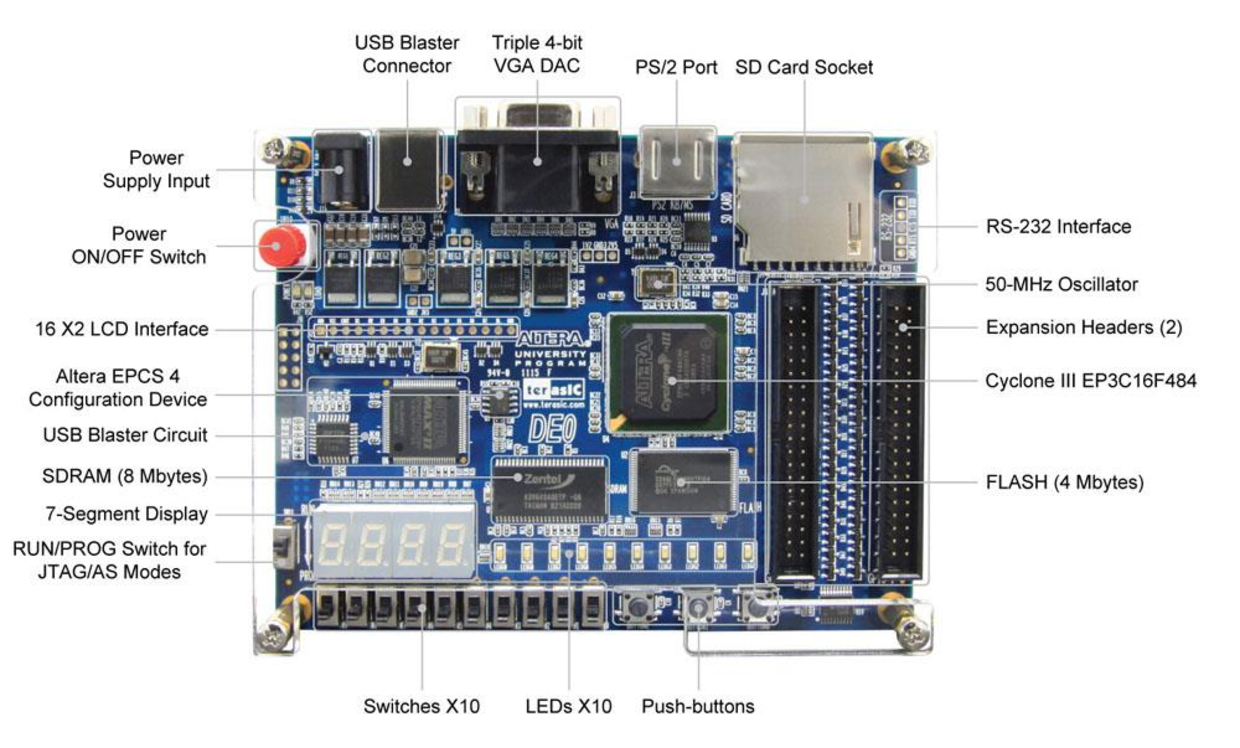
\includegraphics[scale=0.7]{./img/fpga_cycloneIII.pdf}
			\caption{FPGA Cyclone III}
			\label{fig:FPGA_cycloneIII}
		\end{figure}

	\section*{Raspberry Pi Model 2B}
	\label{sec:raspi_model2b}
	\addcontentsline{toc}{section}{Raspberry Pi Model 2B}
		Raspberry Pi Model 2B è una delle piattaforme embedded più conosciute e utilizzate al mondo. Questa scheda è una scelta ideale per una vasta gamma di progetti, in particolare all'Internet delle cose (IoT).

		\begin{figure}[H]
			\centering
			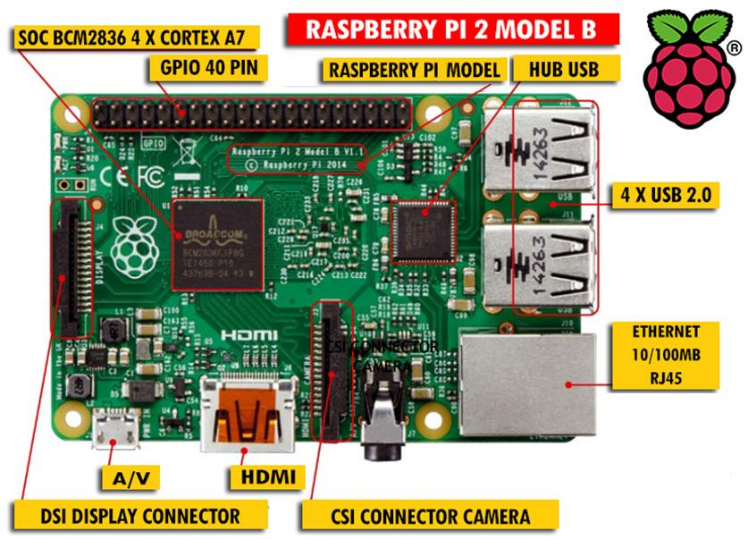
\includegraphics[scale=0.6]{./img/rapi2b.png}
			\caption{Raspberry Pi Model 2B}
			\label{fig:raspi_model2b}
		\end{figure}

		Di seguito le sue specifiche:
		
		\begin{enumerate}
			\item \textbf{Processore:} quad-core ARM Cortex-A7 con clock a 900 MHz;
			
			\item \textbf{Memoria RAM:}  1 GB di memoria RAM;
			\item \textbf{Porte USB:}  4 porte USB 2.0;
			
			\item \textbf{Ethernet:} integrata;
			\item \textbf{HDMI:} supporta l'uscita video Full HD (1080p), consentendo la connessione a monitor e televisori;
			
			\item \textbf{GPIO (General-Purpose Input/Output):} 40 pin GPIO, che consentono di connettere sensori, attuatori e altri dispositivi per vari progetti;
			
			\item \textbf{Alimentazione:} può essere alimentata tramite un adattatore microUSB da 5V;
			
			\item \textbf{Sistema Operativo:}  Linux (come Raspbian), Windows 10 IoT Core e altri.

		\end{enumerate}


\chapter*{Struttura del moltiplicatore 16x16 bit}
\label{ch:struttura_moltiplicatore}
\addcontentsline{toc}{chapter}{Struttura del moltiplicatore 16x16 bit}

	\section*{Come funziona l'algoritmo}
	\label{sec:how_it_works}
	\addcontentsline{toc}{section}{Come funziona l'algoritmo}
		L'algoritmo di moltiplicazione 16x16 bit, si compone di vari passaggi per ottenere il risultato desiderato.
		
		Considerando due operandi \textit{A} e \textit{B} di 16 bit ciascuno, essi verranno scomposti in due parti più piccole, da 8 bit ciascuno come segue: 

		\begin{figure}[ht]
			\centering
			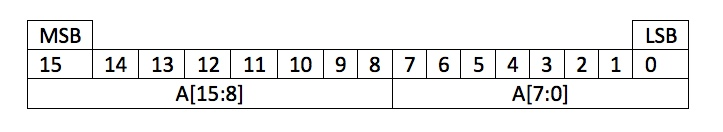
\includegraphics[scale=0.4]{./img/operand-16-bit.jpeg}
			\caption{Suddivisione dell'operando A}
			\label{fig:operando_a}
		\end{figure}

		Successivamente, i passi di moltiplicazione sono suddivisi in operazioni più gestibili. Le operazioni coinvolgono la moltiplicazione tra le parti alte di A e B, la moltiplicazione tra le parti basse di A e B, e varie somme di prodotti intermedi.

		Per comprendere meglio i passaggi, scomponiamo i due operandi come segue:

		\begin{equation}
			A[15:0] = A[15:8]\,\times\,2^8 +A[7:0]\,\times\,2^0
			B[15:0] = B[15:8]\,\times\,2^8 +B[7:0]\,\times\,2^0	
			\label{eq:operandi}	
		\end{equation}
		
		A questo punto se consideriamo di effetturare la moltiplicazione tra gli operandi, si ottiene:
		\begin{equation}
			\footnotesize
			\label{eq:multiply_16x16}
			\begin{aligned}
				A[15:0]\,\times\,B[15:0] &= (A[15:8]\,\times\,2^8\,+\,A[7:0]\,\times\,2^0)\,\times\,(B[15:8]\,\times\,2^8\,+\,B[7:0]\,\times\,2^0) \\ 
				&= A[15:8]\,\times\,B[15:8]\,\times\,2^{16}\,+\,(A[15:8]\,\times\,B[7:0]\,+\,A[7:0]\,\times\,B[15:8])\,\times\,2^8\,+\,A[7:0]\,\times\,B[7:0]
			\end{aligned}
		\end{equation}

		Dall'equazione \ref{eq:multiply_16x16} si ottiene l'algoritmo implementato, dove vengono effettuate più moltiplicazioni, in cascata tra le parti scomposte degli operandi, e sommate sequenzialmente. In figura \ref{fig:multiplier16x16_surfvhdl} viene mostrato uno schema a blocchi della soluzione poroposta.
	
		L'intero processo sfrutta sia la proprietà distributiva che le proprietà delle potenze di 2, come l'espansione di 256 come $2^8$. Questo consente di semplificare le operazioni complesse e ridurre il carico computazionale. \par

		\begin{figure}[H]
			\centering
			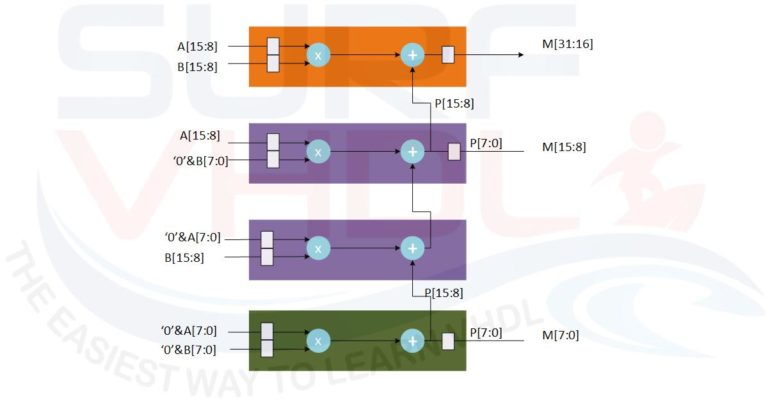
\includegraphics[scale=0.8]{./img/multiplier_16x16_break.jpg}
			\caption{Schema a blocchi della moltiplicazione.}\textit{fonte:} \hyperlink{https://surf-vhdl.com}{surf-vhdl.com}
			\label{fig:multiplier16x16_surfvhdl}
		\end{figure}

		Una moltiplicazione binaria generalmente è svolta eseguendo una serie di somme e prodotti parziali. Dal punto di vista della logica combinatoria si mette in and il moltiplicando con i diversi bit del moltiplicatore, se il moltiplicatore è composto da n bit si hanno n prodotti parziali potenziali ognuno dei quali richiede una somma per costruire il risultato. Avere in posizioni diverse i bit del moltiplicatore da considerare implica che il moltiplicando deve essere opportunamente "\textit{shiftato}": ogni posizione ha peso doppio, quindi si moltiplica per due e questo comporta lo spostamento del prodotto parziale di una posizione a sinistra per ogni bit in più.
		Questo approccio nel caso in cui si stia lavorando con dei numeri binari di grande dimensione
		comporta uno sforzo computazionale elevato.
		
		Esempio: $10100_2\,\times\,11100_2$

		% Tabella in latex
		\begin{table}[h!]
			\centering
			\begin{tabular}{*{11}{p{0.5cm}}}
					&  &  &  &  & 1 & 0 & 1 & 0 & 0 & $\times$  \\
					&  &  &  &  & 1 & 1 & 1 & 0 & 0 & $=$ \\
				\cline{1-11}
				& & & &  & 0 & 0 & 0 & 0 & 0 & $+$ \\
				& & & & 0 & 0 & 0 & 0 & 0 &  & $+$ \\
				& &  & 1 & 0 & 1 & 0 & 0 &  &  & $+$ \\
				& & 1 & 0 & 1 & 0 & 0 &   &  &  & $+$ \\
			 	& 1 & 0 & 1 & 0 & 0 &   &   &  &  & $=$ \\
				\cline{1-11}
				 1 & 0 & 0 & 0 & 1 & 1 & 0 & 0 & 0 & 0 & \\
			\end{tabular}
			\caption{Esempio di moltiplicazione binaria}
			\label{tab:es_mult_bin}
		\end{table}
	\section*{Descrizione dell'algoritmo di moltiplicazione}
	\label{sec:algoritmo_moltiplicazione}
	\addcontentsline{toc}{section}{Descrizione dell'algoritmo di moltiplicazione}
		L'entity VHDL \textbf{mult\_sgn\_break\_16x16} implementa un moltiplicatore a 16 bit che prende in input due operandi, \textit{i\_ma} e \textit{i\_mb}, e produce in output il risultato della moltiplicazione, \textit{o\_m}, rappresentato su 32 bit.

		Il moltiplicatore utilizza una struttura scomposta per calcolare il prodotto tra i due operandi. Il processo principale, denominato \textit{p\_mult}, è sensibile ai segnali di clock (\textit{i\_clk}) e di reset (\textit{i\_rstb}). Durante la fase di reset, tutti i segnali intermedi vengono inizializzati a zero per garantire un corretto avvio del modulo.
		
		Il calcolo della moltiplicazione avviene all'interno del processo \textit{p\_mult}. I segnali intermedi (\textit{r\_ma\_hi}, \textit{r\_ma\_lo}, \textit{r\_mb\_hi}, \textit{r\_mb\_lo}, \textit{r\_m\_hi}, \textit{r\_m\_md}, \textit{r\_m\_lo}, \textit{r\_m}) vengono utilizzati per memorizzare i valori intermedi durante il calcolo (vedi Listato~\ref{lst:mul16_process}).
		
		\begin{lstlisting}[caption={\textbf{mul16.vhd} - architettura del motiplicatore a 16 bit}, label={lst:mul16_process}]
-------------------------------------------------
-- Project : Moltiplicatore a 16bit            --
-- Author :  Brescia Luca                      -- 
--           Loda Michele                      --
--           Pezzottini Simone                 --
-- Date : AY2022/2023                          --
-- Company : UniBS                             --
-- File : mul16.vhd                            --
-------------------------------------------------

library ieee;
use ieee.std_logic_1164.all;
use ieee.numeric_std.all;

entity mult_sgn_break_16x16 is
	generic (
		NUM_CYCLES : integer := 16 --! Numero di cicli per effettuare la moltiplicazione
	);
	port ( 
		i_clk  : in  std_logic;
		i_rstb : in  std_logic;
		i_en   : in  std_logic;
		i_ma   : in  std_logic_vector(15 downto 0);
		i_mb   : in  std_logic_vector(15 downto 0);
		o_m    : out std_logic_vector(31 downto 0);
		o_rdy  : out std_logic								--! output ready
	);
end mult_sgn_break_16x16;

architecture rtl of mult_sgn_break_16x16 is

	-- Segnali intermedi per il calcolo della moltiplicazione
	signal r_ma_hi  : signed(7 downto 0);   -- Parte alta del primo operandi (A[15:8])
	signal r_ma_lo  : signed(8 downto 0);   -- Parte bassa del primo operandi con bit di segno (A[7:0])
	signal r_mb_hi  : signed(7 downto 0);   -- Parte alta del secondo operandi (B[15:8])
	signal r_mb_lo  : signed(8 downto 0);   -- Parte bassa del secondo operandi con bit di segno (B[7:0])
	signal r_m_hi   : signed(15 downto 0);  -- Moltiplicazione tra parti alte (A[15:8] * B[15:8])
	signal r_m_md   : signed(16 downto 0);  -- Moltiplicazione tra parti alte e basse sommate (A[15:8] * B[7:0] + A[7:0] * B[15:8])
	signal r_m_lo   : signed(17 downto 0);  -- Moltiplicazione tra parti basse (A[7:0] * B[7:0]) con bit di segno esteso
	signal r_m      : signed(31 downto 0);  -- Risultato della moltiplicazione finale
	signal counter  : integer;              -- contatore cicli di clock

begin
	o_m <= std_logic_vector(r_m);  -- Assegnamento del risultato alla porta di output o_m

	-- Calcolo della moltiplicazione a 16 bit
	r_m_hi <= r_ma_hi * r_mb_hi;
	r_m_md <= r_ma_hi * r_mb_lo + r_mb_hi * r_ma_lo;
	r_m_lo <= r_ma_lo * r_mb_lo;

	p_mult : process(i_clk, i_rstb)
	begin
	if (i_rstb = '1') then
		-- Reset dei segnali intermedi
		r_ma_hi <= (others => '0');
		r_ma_lo <= (others => '0');
		r_mb_hi <= (others => '0');
		r_mb_lo <= (others => '0');
		r_m     <= (others => '0');
		counter <= 0;
		o_rdy   <= '0';
	elsif (rising_edge(i_clk)) then
		if i_en = '1' then
		-- Assegnazione dei valori ai segnali intermedi durante il ciclo di clock
		r_ma_hi <= signed(i_ma(15 downto 8));      -- Assegnazione della parte alta del primo operandi
		r_ma_lo <= signed('0' & i_ma(7 downto 0)); -- Assegnazione della parte bassa del primo operandi con estensione del bit di segno
		r_mb_hi <= signed(i_mb(15 downto 8));      -- Assegnazione della parte alta del secondo operandi
		r_mb_lo <= signed('0' & i_mb(7 downto 0)); -- Assegnazione della parte bassa del secondo operandi con estensione del bit di segno
		r_m     <= r_m_hi & "0000000000000000" + resize(r_m_md & "00000000", 32) + resize(r_m_lo, 32);  -- Calcolo del risultato finale della moltiplicazione
		--! Aumento il numero di cicli effettuati per la moltiplicazione, se li supero segnalo output ready
		counter <= counter + 1;
		if counter >= NUM_CYCLES then
			o_rdy <= '1';
		end if;
		else
		counter <= 0;
		o_rdy <= '0';
		end if;
	end if;
	end process p_mult;
end rtl;
		\end{lstlisting}
		
		Il risultato finale della moltiplicazione viene assegnato alla porta di output \textit{o\_m} come una stringa binaria convertita in un vettore di segnali di tipo \textit{std\_logic\_vector}.
		
		Il modulo VHDL \textbf{mul16} è stato progettato per eseguire moltiplicazioni a 16 bit in modo efficiente e preciso, fornendo un'implementazione hardware ottimizzata per l'FPGA Cyclone III EP3C16F484C6.
		
		\subsection*{Motivazioni della dimensione dei dati}
		\label{subsec:scelta_dimensione_dati}
		\addcontentsline{toc}{subsection}{Motivazioni della dimensione dei dati}
			Nel progetto del moltiplicatore a 16 bit, la scelta della dimensione dei dati influisce sull'ottimizzazione delle prestazioni e nell'occupazione delle risorse. La dimensione dei dati si riferisce alla quantità di bit utilizzati per rappresentare i valori di input e output del moltiplicatore.

			Una dimensione di 16 bit permette di gestire una vasta gamma di numeri interi senza introdurre una complessità eccessiva. I dati a 16 bit possono rappresentare valori compresi tra $-2^{15}$ e $2^{15}-1$. Nel contesto di un moltiplicatore, è spesso necessario eseguire operazioni su numeri relativamente piccoli, ma con una precisione sufficiente per evitare overflow o underflow.

			Dimensioni maggiori dei dati potrebbero richiedere risorse hardware aggiuntive, aumentando il consumo energetico e la latenza.
			Infine, le operazioni aritmetiche e logiche su dati a 16 bit sono ben supportate dalle librerie standard del linguaggio VHDL, semplificando il processo di sviluppo e di debugging.


\chapter*{Progettazione e implementazione in VHDL}
\label{ch:progettazione_vhdl}
\addcontentsline{toc}{chapter}{Progettazione e implementazione in VHDL}
	\section*{Descrizione del linguaggio VHDL}
	\label{sec:desc_vhdl}
	\addcontentsline{toc}{chapter}{Descrizione del linguaggio VHDL}
		Il VHDL (\textit{VHSIC Hardware Description Language}) è un linguaggio di descrizione hardware utilizzato per descrivere circuiti digitali complessi.

		Il linguaggio permette di modellare il comportamento e la struttura dei circuiti, consentendo di sviluppare soluzioni hardware in modo efficiente.

		Le principali caratteristiche del VHDL includono:
		\begin{itemize}
			\item \textbf{Descrizione Comportamentale:} Il VHDL consente di definire il comportamento di un circuito attraverso processi. Questi processi contengono istruzioni sequenziali che modellano l'evoluzione del circuito nel tempo.
			
			\item \textbf{Descrizione Strutturale:} È possibile definire la struttura di un circuito attraverso la connessione di componenti predefiniti. Questo approccio permette di creare circuiti complessi combinando blocchi più semplici.
			
			\item \textbf{Tipi di Dati:} VHDL offre una vasta gamma di tipi di dati, tra cui booleani, interi, vettori e record. Questi tipi consentono di modellare sia segnali digitali che dati analogici.
			
			\item \textbf{Sintassi Gerarchica:} È possibile definire circuiti a più livelli di gerarchia, suddividendo la progettazione in moduli più piccoli e riutilizzabili.
			
			\item \textbf{Simulazione:} Uno dei vantaggi chiave del VHDL è la possibilità di eseguire simulazioni per verificare il comportamento del circuito prima della fase di implementazione hardware.
		\end{itemize}

		Il processo di sviluppo in VHDL inizia con la definizione dei moduli e dei componenti necessari. Questi moduli vengono collegati tra loro per creare il circuito completo. Successivamente, vengono scritti processi per descrivere il comportamento dei singoli moduli.

		Una volta completata la descrizione in VHDL, è possibile eseguire simulazioni per testare il funzionamento del circuito in diverse condizioni. Questo approccio aiuta a individuare errori e problemi prima della fase di implementazione hardware.

		In conclusione, il VHDL è uno strumento potente per la progettazione di circuiti digitali. La sua combinazione di descrizione comportamentale e strutturale, insieme alla capacità di simulazione, lo rende uno strumento essenziale nell'industria dell'elettronica digitale.
	\section*{Codice implementato}
	\label{sec:vhdl_code}
	\addcontentsline{toc}{section}{Codice implementato}
		
		L'architettura \texttt{basic\_mult} rappresenta il top level dell'architettura implementata. Essa costituisce un sistema in cui diverse entità lavorano sinergicamente per realizzare l'obiettivo complessivo del progetto.
		Gestisce l'interconnessione tra entità, tra cui i componenti personalizzati e i moduli predefiniti fornitici durante il corso.
		
		Il modulo \texttt{spi}, che abilita l'interfacciamento tra dispositivi attraverso una comunicazione seriale sincrona. Questo modulo viene utilizzato per stabilire una comunicazione con dispositivi esterni. Nel nostro caso, con la scheda di sviluppo \textit{RaspberryPi}.

		Parimenti, il modulo \texttt{blink heartbeat} è un'entità, fornita durante il corso, che non richiede modifiche significative all'integrazione. Esso fornisce un indicatore visivo dello stato operativo del sistema tramite il lampeggio di un LED.

		L'integrazione delle vaire entità all'interno dell'architettura \texttt{basic\_mult} richiede la sincronizzazione dei segnali di controllo, flussi di dati e temporizzazioni.
		Per questo motivo è stata creata una macchina a stati che regola il funzionamento del sistema. Le varie connessioni tra le entity garantiscono la propagazione del segnale una volta che viene abilitato dalla macchina a stati.

		Essa si suddivide in due signal:
		\begin{enumerate}
			\item \texttt{current state}: stato corrente della macchina a stati;
			\item \texttt{next state}: stato successivo della macchina a stati, valorizzato al verificarsi di una condizione ben precisa.
		\end{enumerate}

		Inoltre, sono stati creati vari processi che, parallelamente, gestiscono il funzionamento del sistema completo.

		Di seguito, viene riportato per intero il codice dell'entity \texttt{basic\_mult}, che costituisce il top-level per la nostra architettura.

		\begin{lstlisting}[caption={Top level implementato per la nostra architettura}, label={lst:mul16_process}]
-------------------------------------------------
-- Project : Moltiplicatore a 16bit            --
-- Author :  Brescia Luca                      -- 
--           Loda Michele                      --
--           Pezzottini Simone                 --
-- Date : 	 AY2022/2023                       --
-- Company : UniBS                             --
-- File : 	 basic_mult.vhd       		        --
-------------------------------------------------

library IEEE;

use IEEE.STD_LOGIC_1164.all;
use IEEE.NUMERIC_STD.all;

entity basic_mult is
	port
	(
	CLOCK_50 : in std_logic;                        --! Clock di sistema a 50 MHz
	KEY      : in std_logic_vector(2 downto 0);     --! Segnali di controllo push buttons
	LEDG     : out std_logic_vector(9 downto 0);    --! Segnali di output per i LED
	GPIO_1   : inout std_logic_vector(31 downto 0)  --! Segnali di input/output GPIO
	);
end basic_mult;

architecture top_arch of basic_mult is
	--! Definizioni costanti
	constant DATA_W         : integer := 32;  --! Dimensione del dato
	constant Nbit           : integer := 5;   --! Numero di bit per contenere il dato
	constant all_zeros      : std_logic_vector(DATA_W - 1 downto 0) := (others => '0');      --! Dati in ingresso SPI
	--! Stati per la macchina a stati
	type my_states is (STATE_WAIT_NEW_DATA, STATE_START_MULTIPLY, STATE_MULT_READY, STATE_DATA_SENT); --! Stati possibili per la macchina a stati
	signal current_state : my_states;   --! Stato corrente della macchina a stati
	signal next_state: my_states;       --! Prossimo stato della macchina a stati
	--! Definizioni signals
	signal pb0_synchronizer : std_logic_vector(2 downto 0);               --! Sincronizzatore del pushbutton per segnale di reset
	signal SYS_SPI_SCK      : std_logic                          := '0';  --! Pin di clock SPI
	signal SYS_SPI_MOSI     : std_logic                          := '0';  --! Pin di output dati SPI
	signal SYS_SPI_MISO     : std_logic                          := '0';  --! Pin di input dati SPI
	signal spi_data_in      : std_logic_vector(DATA_W - 1 downto 0);      --! Dati in ingresso SPI
	signal spi_data_out     : std_logic_vector(DATA_W - 1 downto 0);      --! Dati in uscita SPI
	signal mult_data_a      : std_logic_vector(DATA_W/2 - 1 downto 0);    --! Copia del dato in ingresso
	signal mult_data_b      : std_logic_vector(DATA_W/2 - 1 downto 0);    --! Copia del dato in ingresso
	signal result           : std_logic_vector(DATA_W - 1 downto 0);      --! Risultato della moltiplicazione
	signal reset            : std_logic                         := '0';   --! Flag di reset
	signal enable_clk       : std_logic                         := '0';   --! Flag di abilitazione clock per l'entity moltiplicatore
	signal newdata          : std_logic                         := '0';   --! Flag di presenza nuovo dato da inviare
	signal multready        : std_logic                         := '0';   --! Flag di segnalazione dato moltiplicato corretto
	signal datasent         : std_logic                         := '0';   --! Flag di invio corretto del dato

begin
	--! Assegnazione dei segnali SPI ai pin fisici GPIO
	SYS_SPI_SCK  <= GPIO_1(7);  --! Segnale di clock spi
	SYS_SPI_MOSI <= GPIO_1(5);  --! Segnale di input per FPGA (Slave)
	GPIO_1(3) <= SYS_SPI_MISO;  --! Segnale di output per FPGA (Slave)
	
	--! Gestione del lampeggio del LED 
	blink_hb : entity work.blink_heartbeat port map(
	CLK => CLOCK_50,
	LED => LEDG(0)
	);

	--! Istanza del modulo SPI
	spi_inst : entity work.spi
	generic
	map (
	DATA_W => 32,
	Nbit   => 5
	)
	port
	map (
	CLK      => CLOCK_50,
	reset    => reset,
	DATA_IN  => spi_data_out,
	DATA_OUT => spi_data_in,
	RD       => datasent,
	WR       => newdata,
	SCK      => SYS_SPI_SCK,
	MOSI     => SYS_SPI_MOSI,
	MISO     => SYS_SPI_MISO
	);

	--! Istanza del moltiplicatore 16x16
	mult_inst : entity work.mult_sgn_break_16x16
	port
	map (
	i_clk  => CLOCK_50,
	i_rstb => reset,
	i_en   => enable_clk,
	i_ma   => mult_data_a,
	i_mb   => mult_data_b,
	o_m    => result,
	o_rdy  => multready
	);

	--! Processo principale per la gestione della macchina a stati per la realizzazione del moltiplicatore senza segno spi
	--! Attende un dato in ingresso su spi formattato come segue: (MOLTIPLICATORE << 16 | MOLTILPICANDO) dove moltiplicando e moltiplicatore sono due interi senza segno a 16 bit
	main_process : process (current_state, newdata, multready, datasent)
	begin
	--! Gestione della macchina a stati
	case current_state is
		--! Attesa del nuovo dato
		when STATE_WAIT_NEW_DATA =>
			enable_clk <= '0';                    --! Reset clk dell'istanza moltiplicatore
			LEDG(9 downto 2) <= (others => '0');  --! Reset dei led presenti su FPGA
		next_state <= STATE_WAIT_NEW_DATA;
			--! Controllo presenza flag di nuovo dato e che il dato sia diverso da 0
			if newdata = '1' and (spi_data_in /= all_zeros) then
			--! Divisione del dato di ingresso a 32bit come dato_a e dato_b
			mult_data_a <= spi_data_in(15 downto 0);  --! Moltiplicando parte bassa (0 - 15) del dato in ingresso
			mult_data_b <= spi_data_in(31 downto 16); --! Moltiplicatore parte alta (16- 31) del dato in ingresso
			next_state <= STATE_START_MULTIPLY;       --! Avanzamento di stato della macchina a stati
			end if;

		--! Avvio moltiplicazione e attesa completamento
		when STATE_START_MULTIPLY =>
			enable_clk <= '1';  --! Abilitazione del segnale di clock per la entity mult_sgn_break_16x16
		next_state <= STATE_START_MULTIPLY;
			--! Attesa flag moltiplicazione terminata
			if multready = '1' then
			spi_data_out <= result;           --! Copia del risultato sul signal che inviera' su spi il valore
			next_state <= STATE_MULT_READY;   --! Avanzamento di stato della macchina a stati
			end if;

		--! Moltiplicazione completata e attesa di fine invio del dato su spi
		when STATE_MULT_READY =>
			enable_clk <= '0'; --! Arresto del segnale di clock per la entity mult_sgn_break_16x16
			next_state <= STATE_MULT_READY; 
			--! Attesa flag dato inviato
			if datasent = '1' then
			next_state <= STATE_DATA_SENT;    --! Avanzamento di stato della macchina a stati
			end if;

		--! Termine delle operazioni
		when STATE_DATA_SENT =>
		LEDG(7) <= '1'; --! Segnalazione tramite accensione del led7 delle operazioni concluse
	next_state <= STATE_DATA_SENT;--! Loopback del nuovo stato
		--! Se il flag di dato inviato e' attivo
		if datasent = '1' then
			LEDG(8) <= '1'; --! Segnalazione tramite accensione del led8 del corretto invio del dato
		end if;
		when others =>
			LEDG(9) <= '1'; --! Segnalazione tramite accensione del led9 della metastabilita'
	end case;
	end process;

	--! Gestione dell'avanzamento di stato della macchina a stati
	state_memory : process (CLOCK_50, reset) --! Stati possibili per la macchina a stati
	begin
	--! Gestione del segnale di reset
	if reset = '1' then
		current_state <= STATE_WAIT_NEW_DATA;    --! Reset macchina a stati
	elsif (rising_edge(CLOCK_50)) then
		current_state <= next_state;			     --! Avanzamento di stato
	end if;
	end process;
	
	--! Gestione del segnale di reset
	reset_handle : process (CLOCK_50, KEY)
	begin
	--! Trigger delle operazioni sul fronte positivo del clock FPGA
	if (rising_edge(CLOCK_50)) then
		--! Sincronizzazione del pushbutton0 e generazione del segnale di reset
		pb0_synchronizer(2 downto 1) <= pb0_synchronizer(1 downto 0);
		pb0_synchronizer(0)          <= KEY(0);

		--! Fronte positivo indica che il pushbutton0 e' stato rilasciato
		if pb0_synchronizer(2 downto 1) = "01" then
		LEDG(1) <= '1';   --! Segnalazione tramite accensione del led1 l'attivazione del segnale di reset
		reset   <= '1';   --! Attivazione segnale di reset
		--! Se e' stato attivato al clock precedente il segnale di reset
		elsif (reset = '1') then
		LEDG(1) <= '0';   --! Segnalazione tramite spegnimento del led1 la disattivazione del segnale di reset
		reset   <= '0';   --! Disattivazione segnale di reset
		end if;
	end if;
	end process;
end top_arch;
		\end{lstlisting}
		\subsection*{Approccio di progettazione}
		\label{subsec:approccio_progettazione}
		\addcontentsline{toc}{subsection}{Approccio di progettazione}
			La scelta di implementare una macchina a stati per gestire il processo di moltiplicazione all'interno del progetto è motivata dalla necessità di coordinare e controllare le diverse fasi coinvolte nel funzionamento del progetto. La moltiplicazione in sé è un'operazione complessa che richiede diverse fasi di calcolo, sincronizzazione e gestione dei segnali di controllo. Inoltre, in questo progetto viene richiesto il corretto funzionamento della comunicazione SPI, da cui bisogna ottenere i due operandi e inviare successivamente il risultato della loro moltiplicazione.

			La macchina a stati offre un'organizzazione strutturata per gestire queste diverse fasi in modo sequenziale e controllato. Ciascuno stato rappresenta una fase specifica del processo di funzionamento, consentendo una suddivisione chiara e modulare delle operazioni coinvolte. Questo approccio non solo semplifica la progettazione e l'implementazione, ma contribuisce anche a una maggiore comprensione del flusso di lavoro.

			In particolare, con riferimento al listato \ref*{lst:mul16_process}:
			
			\begin{itemize}
				\item \texttt{STATE\_WAIT\_NEW\_DATA} è lo stato responsabile della lettura dei dati in ingresso. Il sistema resta in questo stato finché non viene segnalata la presenza di un nuovo dato di ingresso \emph{newdata} con l'aggiunta del controllo che sia diverso da zero. Questo stato è anche lo stato indotto dal segnale di reset.
				\item \texttt{STATE\_START\_MULTIPLY} è lo stato indotto dopo che è stato correttamente ricevuto un dato da SPI. Avvia il processo di moltiplicazione attivando il clock corrispondente all'entity \emph{mult\_inst} e attende il segnale \emph{o\_rdy} corrispondente alla presenza del dato moltiplicato correttamente.
				\item \texttt{STATE\_MULT\_READY} è lo stato indotto dopo che la moltiplicazione è terminata. Esso avvia il processo di invio del dato tramite l'entity \textit{spi\_inst} e attende finché non è segnalato il corretto invio del dato.
				\item \texttt{STATE\_DATA\_SENT} è lo stato indotto quando il dato è stato correttamente inviato. Esso segna la fine di tutte le operazioni. Il sistema resta in questo stato di \textit{IDLE} finché un nuovo segnale di reset non è ricevuto.
			\end{itemize} 

			Ogni transizione tra stati è governata da un insieme di condizioni ben definite, che aiuta a garantire che le operazioni avvengano nel momento giusto e con il timing corretto. Ciò è particolarmente importante in un sistema sincrono come quello in questione, dove il corretto sequenziamento delle operazioni è essenziale per ottenere risultati corretti.

\chapter*{Simulazione e verifica}
\label{ch:simulazione_verifica}
\addcontentsline{toc}{chapter}{Simulazione e verifica}
	\section*{Introduzione alla Simulazione con Altera ModelSim per l'Architecture "basic\_mult"}
	\label{sec:intro_sim_modelsim}			
	\addcontentsline{toc}{chapter}{Introduzione alla Simulazione con Altera ModelSim per l'Architecture "basic\_mult"}
		La simulazione è un passo cruciale nel processo di progettazione hardware, poiché consente di verificare il funzionamento e l'interazione delle diverse componenti del sistema. Nel contesto del progetto basato sull'architecture "basic\_mult", l'obiettivo è quello di realizzare un moltiplicatore a 16 bit. Per verificare l'effettivo funzionamento di tale componente, è stato utilizzato l'ambiente di simulazione Altera ModelSim. \par

		Di seguito viene riportato il codice utilizzato per la creazione del testbench:
		
		\begin{lstlisting}[caption={Test bench dell'architettura \textit{basic\_mult}}, label={lst:tb_spi.vhd}]
-------------------------------------------------
-- Project : Moltiplicatore a 16bit            --
-- Author :  Brescia Luca                      -- 
--           Loda Michele                      --
--           Pezzottini Simone                 --
-- Date : AY2022/2023                          --
-- Company : UniBS                             --
-- File : tb_spi.vhd           		             --
-------------------------------------------------
library ieee;
use ieee.std_logic_1164.all;
use ieee.numeric_std.all;

entity tb_spi is
end tb_spi;

architecture sim of tb_spi is
	COMPONENT testbench
	port
	(
		CLOCK_50 : in std_logic;                        --! Clock di sistema a 50 MHz
		SW       : in std_logic_vector(9 downto 0);     --! Dati in ingresso da interruttore
		KEY      : in std_logic_vector(2 downto 0);     --! Segnali di controllo push buttons
		LEDG     : out std_logic_vector(9 downto 0);    --! Segnali di output per i LED
		GPIO_1   : inout std_logic_vector(31 downto 0)  --! Segnali di input/output GPIO
	);
	END COMPONENT;

	-- COSTANTI
	constant clk_period:  integer := 20;    -- ns
	constant sck_period:  integer := 200;   -- ns
	constant data1:       integer := 131143;-- max 65535
	constant data2:       integer := 18;    -- max 65535
	constant DATA_W:      integer := 32;    -- dimensione del dato
	constant Nbit:        integer := 5;     -- numero di bit per contenere il dato


	--inout
	signal GPIO_1		: std_logic_vector(DATA_W-1 downto 0);
	
	--Inputs
	signal CLOCK_50		: std_logic:= '0';
	signal KEY			: std_logic_vector(2 downto 0):= (others => '0');
	signal SW			: std_logic_vector(9 downto 0):= (others => '0');	-- Array switch
	signal LEDG			: std_logic_vector(9 downto 0);

	signal reset:       std_logic := '0';
	signal reset_sim:   std_logic := '1';
	signal SCK:         std_logic := '0';
	signal stop_SCK:    boolean   := true;
	signal MOSI:        std_logic := '0';
	signal MISO:        std_logic := '0';
	signal wr_local: std_logic    := '0';
	signal data_in:     std_logic_vector(DATA_W-1 downto 0);
	signal data_out:    std_logic_vector(DATA_W-1 downto 0);
	
	


begin
	SCK  <= GPIO_1(7);  --! Segnale di clock spi
	MOSI <= GPIO_1(5);  --! Segnale di input per FPGA (Slave)
	MISO <= GPIO_1(3);
	dut: entity work.basic_mult
	port map (
		CLOCK_50 => CLOCK_50,
		SW => SW,
		KEY => KEY,
		LEDG => LEDG,
		GPIO_1 => GPIO_1  
	);

	sim_spi: entity work.send_bits
	generic map (
		DATA_W => DATA_W,
		Nbit => Nbit
	)
	port map (
		clk => GPIO_1(7),
		reset => reset_sim,
		bit_out => GPIO_1(5),
		data_out => data_out,
		bit_in => GPIO_1(3),
		data_in => data_in,
		ready => wr_local
		);
		
	process
	begin
	reset <= '1';
	reset_sim <= '1';
	wait for 20 ns;
	reset <= '0';
	reset_sim <= '0';
	wait for 20 ns;

	-- invio mcand = 3000 (0x0BB8)
	data_out <= std_logic_vector(to_unsigned(data1, DATA_W));
	
	stop_SCK <= false;
	reset_sim <= '0';
	wait until wr_local = '1';

	stop_SCK <= true;
	reset_sim <= '1';
	wait for 200 ns;

	data_out <= std_logic_vector(to_unsigned(0, DATA_W));

	stop_SCK <= false;
	reset_sim <= '0';
	wait until wr_local = '1';

	stop_SCK <= true;
	reset_sim <= '1';
	wait for 200 ns;

	stop_SCK <= false;
	reset_sim <= '0';
	wait until wr_local = '1';

	stop_SCK <= true;
	reset_sim <= '1';
	wait for 200 ns;

	-- visualizzo il risultato
	report "Risultato: " & integer'image(to_integer(unsigned(data_in)));
	
	wait;
	end process;

	process
	constant mWait: integer := clk_period/2;
	constant period: time := mWait * 1 ns;
	begin
	CLOCK_50 <= '0';
	loop
		wait for period;
		CLOCK_50 <= not CLOCK_50;
	end loop;
	end process;

	process
	constant mWait: integer := sck_period/2;
	constant period: time := mWait * 1 ns;
	begin
	GPIO_1(7) <= '0';
	loop
		while not stop_SCK loop
		wait for period;
		GPIO_1(7) <= not GPIO_1(7);
		end loop;
		GPIO_1(7) <= '0';
		wait for period;
	end loop;
	end process;
end sim;

		\end{lstlisting}

		\subsection*{Dettagli dello Script di Simulazione}
		\addcontentsline{toc}{subsection}{Dettagli dello script di simulazione}

			Lo script di simulazione è stato progettato per simulare il funzionamento della moltiplicazione a 16 bit, utilizzando una serie di componenti simulate che rappresentano il comportamento dei segnali e delle interconnessioni tipiche del sistema reale. Il cuore dello script è rappresentato da istanze delle entity "spi" e "mult\_sgn\_break\_16x16", corrispondenti alle parti di comunicazione SPI e moltiplicazione, rispettivamente. Inoltre, è presente un blocco per la gestione del segnale di clock e della linea di clock SCK.

			\subsubsection{Configurazione degli input}

				Per simulare la moltiplicazione a 16 bit, vengono forniti input appropriati ai componenti. I valori da moltiplicare vengono forniti alle entity tramite le porte di input "i\_ma" e "i\_mb". Gli input vengono preparati e inviati al componente di moltiplicazione "mult\_sgn\_break\_16x16".

			\subsubsection{Generazione del segnale di clock}

				La simulazione richiede la generazione di un segnale di clock coerente per sincronizzare le operazioni dei componenti. Uno dei processi presenti nello script si occupa di generare il segnale di clock "clk", che alterna i suoi stati secondo un periodo prestabilito.

			\subsubsection{Simulazione della comunicazione SPI}

				Per simulare la comunicazione SPI, è stata utilizzata l'entity "spi". Viene generata una sequenza di bit da inviare, rappresentata dal segnale "shift\_reg", che viene successivamente trasmesso attraverso le linee MOSI (Master Out Slave In) e MISO (Master In Slave Out). Le operazioni di trasmissione e ricezione dei bit vengono simulate utilizzando il segnale "SCK" come clock per sincronizzare le transizioni.

			\subsubsection{Simulazione della moltiplicazione}

				La moltiplicazione a 16 bit è simulata utilizzando l'entity "mult\_sgn\_break\_16x16". Viene fornito un input appropriato, rappresentato dalle variabili "local\_din1" e "local\_din2", alle porte "i\_ma" e "i\_mb" rispettivamente. Il risultato della moltiplicazione viene salvato nel segnale "local\_dout".

			\subsubsection{Gestione dei segnali di controllo}

				I segnali di controllo, come "wr\_local" e "rd\_local", vengono utilizzati per sincronizzare l'invio e la ricezione dei dati tra le diverse componenti simulate. Questi segnali sono utilizzati per controllare i cicli di lettura e scrittura dei dati.

			\subsubsection{Visualizzazione dei risultati}

				Durante la simulazione, i risultati delle operazioni vengono monitorati e visualizzati attraverso l'uso dell'istruzione "report". In particolare, il risultato della moltiplicazione viene convertito in un valore intero e viene visualizzato sulla console di simulazione.

			\subsubsection{Considerazioni sull'uso di Altera Modelsim}

				L'utilizzo di Altera ModelSim come ambiente di simulazione ha permesso di verificare il corretto funzionamento dell'architecture "basic\_mult" in un ambiente controllato e riproducibile. Lo script di simulazione "tb\_spi.vhd" ha consentito di testare diverse operazioni, come la comunicazione SPI e la moltiplicazione a 16 bit, fornendo un'anteprima delle prestazioni e del comportamento dell'architettura prima della sua effettiva implementazione su dispositivi hardware. Va notato che il codice di simulazione è stato creato ad hoc per questo progetto e il suo funzionamento è stato verificato in ambiente ModelSim.


\chapter*{Sintesi e implementazione}
\label{ch:sintesi_implementazione}
\addcontentsline{toc}{chapter}{Sintesi e implementazione}
	\section*{Modulo basic\_mult}
	\label{sec:modulo_basic_mult}
	\addcontentsline{toc}{section}{Modulo basic\_mult}
		\subsection*{Fase di implementazione}
		\label{subsec:basic_mult_implementazione}
		\addcontentsline{toc}{subsection}{Fase di implementazione}
			L'architettura del moltiplicatore implementata e riportata di seguito, riceve in input il clock del sistema, mediante \textit{signal CLOCK\_50}, il segnale di reset, mediante \textit{KEY} e segnali di comunicazione, mediante i \textit{GPIO\_1(5)} e \textit{GPIO\_1(3)}. In uscita, pilota i \textit{LEDG} e il \textit{GPIO\_1} corrispondente al \textit{MISO} dell'FPGA.

			\begin{figure}[H]
				\centering
				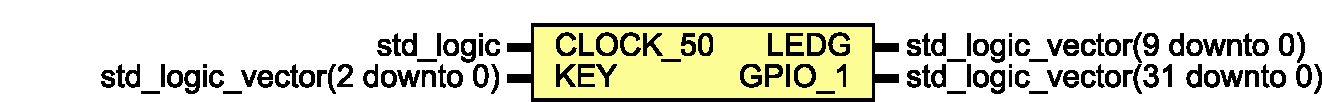
\includegraphics[scale=0.6]{./img/basic_mult_module_teros.pdf}
				\caption{Architettura moltiplicatore implementato}
				\label{fig:basic_mult_module_teros}
			\end{figure}

			Se i \textit{GPIO\_1} sono posizionati nelle uscite nella figura \ref{fig:basic_mult_module_teros} è solamente per un errore di interpretazione del plugin \textit{TerosHDL} poiche i signal \textit{GPIO\_1} sono definiti \texttt{inout}, come riportato in tabella \ref{tab:signal_arch_basic_mult}.

			Di seguito, sono riportati i dettagli dei \textit{signal} utilizzati. I dati riportati sono stati estrapolati dall'output dell'estensione per Visual Studio Code: \textit{TerosHDL}.

			% Tabella in latex
			\begin{table}[H]
			\centering
			\begin{tabular}{|p{0.15\textwidth}|p{0.1\textwidth}|p{0.3\textwidth}|p{0.25\textwidth}|}
				\hline
				\textbf{Nome porta} & \textbf{Direzione} & \textbf{Tipo} & \textbf{Descrizione} \\
				\hline
				CLOCK\_50 & in & std\_logic & Clock di sistema a 50 MHz \\
				KEY & in & std\_logic\_vector(2 downto 0) & Segnali di controllo push buttons \\
				LEDG & out & std\_logic\_vector(9 downto 0) & Segnali di output per i LED \\
				GPIO\_1 & inout & std\_logic\_vector(31 downto 0) & Segnali di input/output GPIO \\
				\hline
			\end{tabular}
			\caption{Segnali del top level dell'architettura}
			\label{tab:signal_arch_basic_mult}
		\end{table}

			% Tabella in latex
			\begin{table}[H]
				\centering
				\begin{tabular}{|p{0.15\textwidth}|p{0.4\textwidth}|p{0.4\textwidth}|}
					\hline
					\textbf{Nome} & \textbf{Tipo} & \textbf{Descrizione} \\
					\hline
					current\_state & my\_states & Stato corrente della macchina a stati \\
					next\_state & my\_states & Prossimo stato della macchina a stati \\
					pb0\_synchronizer & std\_logic\_vector(2 downto 0) & Sincronizzatore del pushbutton per segnale di reset \\
					SYS\_SPI\_SCK & std\_logic & Pin di clock SPI \\
					SYS\_SPI\_MOSI & std\_logic & Pin di output dati SPI \\
					SYS\_SPI\_MISO & std\_logic & Pin di input dati SPI \\
					spi\_data\_in & std\_logic\_vector(DATA\_W - 1 downto 0) & Dati in ingresso SPI \\
					spi\_data\_out & std\_logic\_vector(DATA\_W - 1 downto 0) & Dati in uscita SPI \\
					mult\_data\_a & std\_logic\_vector(DATA\_W/2 - 1 downto 0) & Copia del dato in ingresso \\
					mult\_data\_b & std\_logic\_vector(DATA\_W/2 - 1 downto 0) & Copia del dato in ingresso \\
					result & std\_logic\_vector(DATA\_W - 1 downto 0) & Risultato della moltiplicazione \\
					reset & std\_logic & Flag di reset \\
					enable\_clk & std\_logic & Flag di abilitazione clock per l'entity moltiplicatore \\
					newdata & std\_logic & Flag di presenza nuovo dato da inviare \\
					multready & std\_logic & Flag di segnalazione dato moltiplicato corretto \\
					datasent & std\_logic & \\
					\hline
				\end{tabular}
				\caption{Segnali interni all'architettura \textit{top\_arch} di basic\_mult}
				\label{tab:signal_arch_basic_mult_internal}
			\end{table}

			\begin{table}[H]
				\centering
				\begin{tabular}{|p{0.15\textwidth}|p{0.4\textwidth}|p{0.1\textwidth}|p{0.2\textwidth}|}
					\hline
					\textbf{Nome} & \textbf{Tipo} & \textbf{Valore} & \textbf{Descrizione} \\
					\hline
					DATA\_W & integer & 32 & Dimensione del dato \\
					Nbit & integer & 5 & Numero di bit per contenere il dato \\
					all\_zeros & std\_logic\_vector(DATA\_W - 1 downto 0) & 0 & Dati in ingresso SPI \\
					\hline
				\end{tabular}
				\caption{Costanti utilizzate nell'architettura \textit{top\_arch} di basic\_mult}
				\label{tab:constant_arch_basic_mult_internal}
			\end{table}

			\begin{table}[H]
				\centering
				\begin{tabular}{|p{0.15\textwidth}|p{0.35\textwidth}|}
					\hline
					\textbf{Nome} & \textbf{Tipo} \\
					\hline
					my\_states & STATE\_WAIT\_NEW\_DATA,\newline STATE\_START\_MULTIPLY,\newline STATE\_MULT\_READY,\newline STATE\_DATA\_SENT \\
					\hline
				\end{tabular}
				\caption{Possibili valori per la macchina a stati nell'architettura \textit{top\_arch} di basic\_mult}
				\label{tab:state_arch_basic_mult_internal}
			\end{table}

			La macchina a stati che regola il funzionamento del sistema è la seguente:

			\begin{figure}[H]
				\centering
				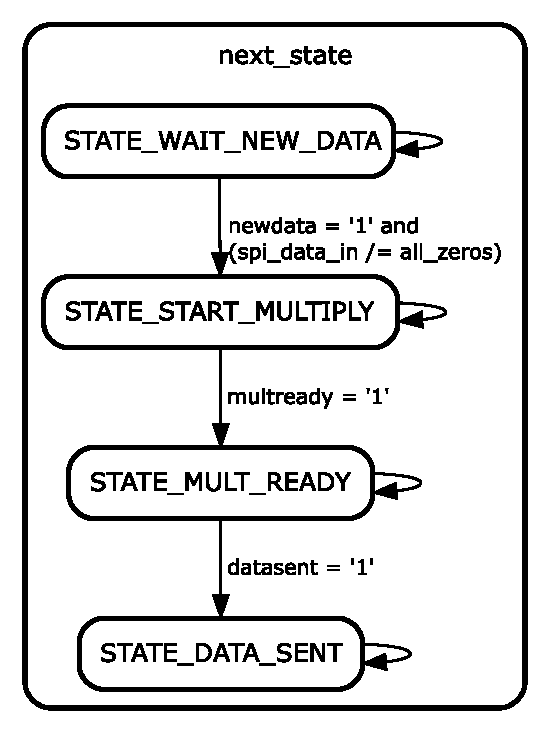
\includegraphics[scale=0.6]{./img/basic_mult_state_machine_0.pdf}
				\caption{Finite state machine ottenuta con l'estensione \textit{TerosHDL}}
				\label{fig:fsm_teros}
			\end{figure}

			Si è verificata la correttezza della macchina a stati esposta in figura \ref*{fig:fsm_teros} ottenendo la visualizzazione della macchina a stati prodotta da \textit{Quartus}:

			\begin{figure}[H]
				\centering
				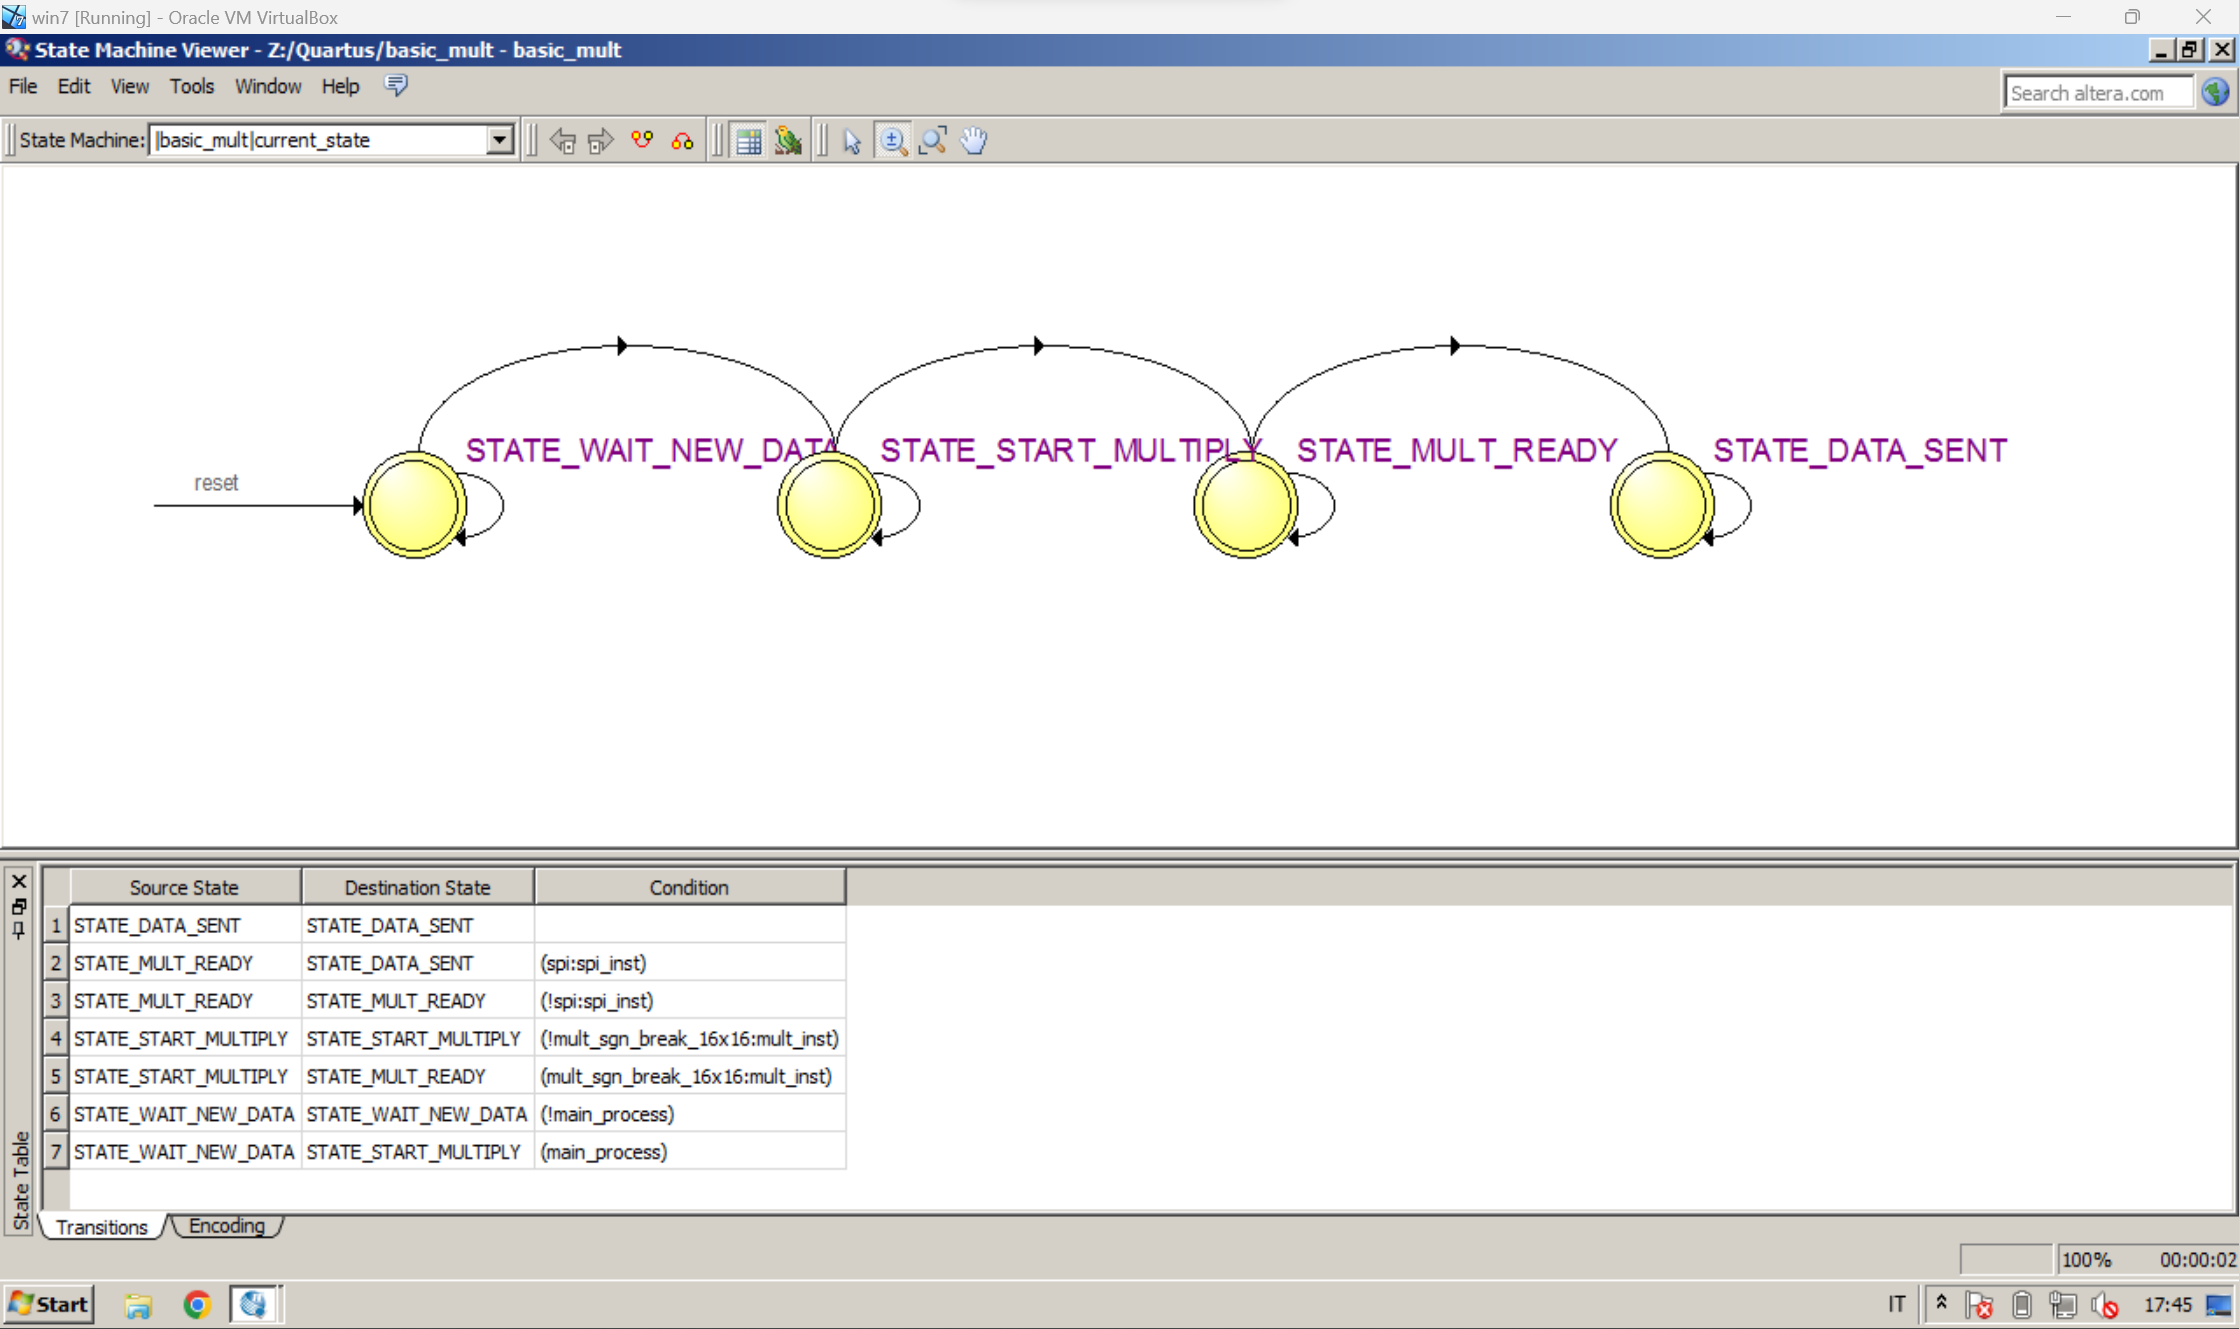
\includegraphics[scale=0.4]{./img/quartus_state_machine.png}
				\caption{Finite state machine ottenuta con \textit{Quartus}}
				\label{fig:fsm_quartus}
			\end{figure}	

			Si può notare dalle figure \ref{fig:fsm_teros} e \ref{fig:fsm_quartus} come le macchine a stati ottenute siano equivalenti.

			In particolare, osservando la figura \ref{fig:fsm_quartus}:

			\begin{itemize}
				\item L'ingresso asincrono della macchina a stati è il comando di \textit{reset};
				\item Gli stati sono quelli sopraelencati nella tabella \ref{tab:state_arch_basic_mult_internal}.
			\end{itemize}
				

		\subsection*{Fase di sintesi}
		\label{subsec:basic_mult_fase_sintesi}
		\addcontentsline{toc}{subsection}{Fase di sintesi}
			
			La vista RTL del moltiplicatore ottenuta da \textit{Quartus} con la compilazione del codice VHDL è la seguente:

			\begin{figure}[H]
				\centering
				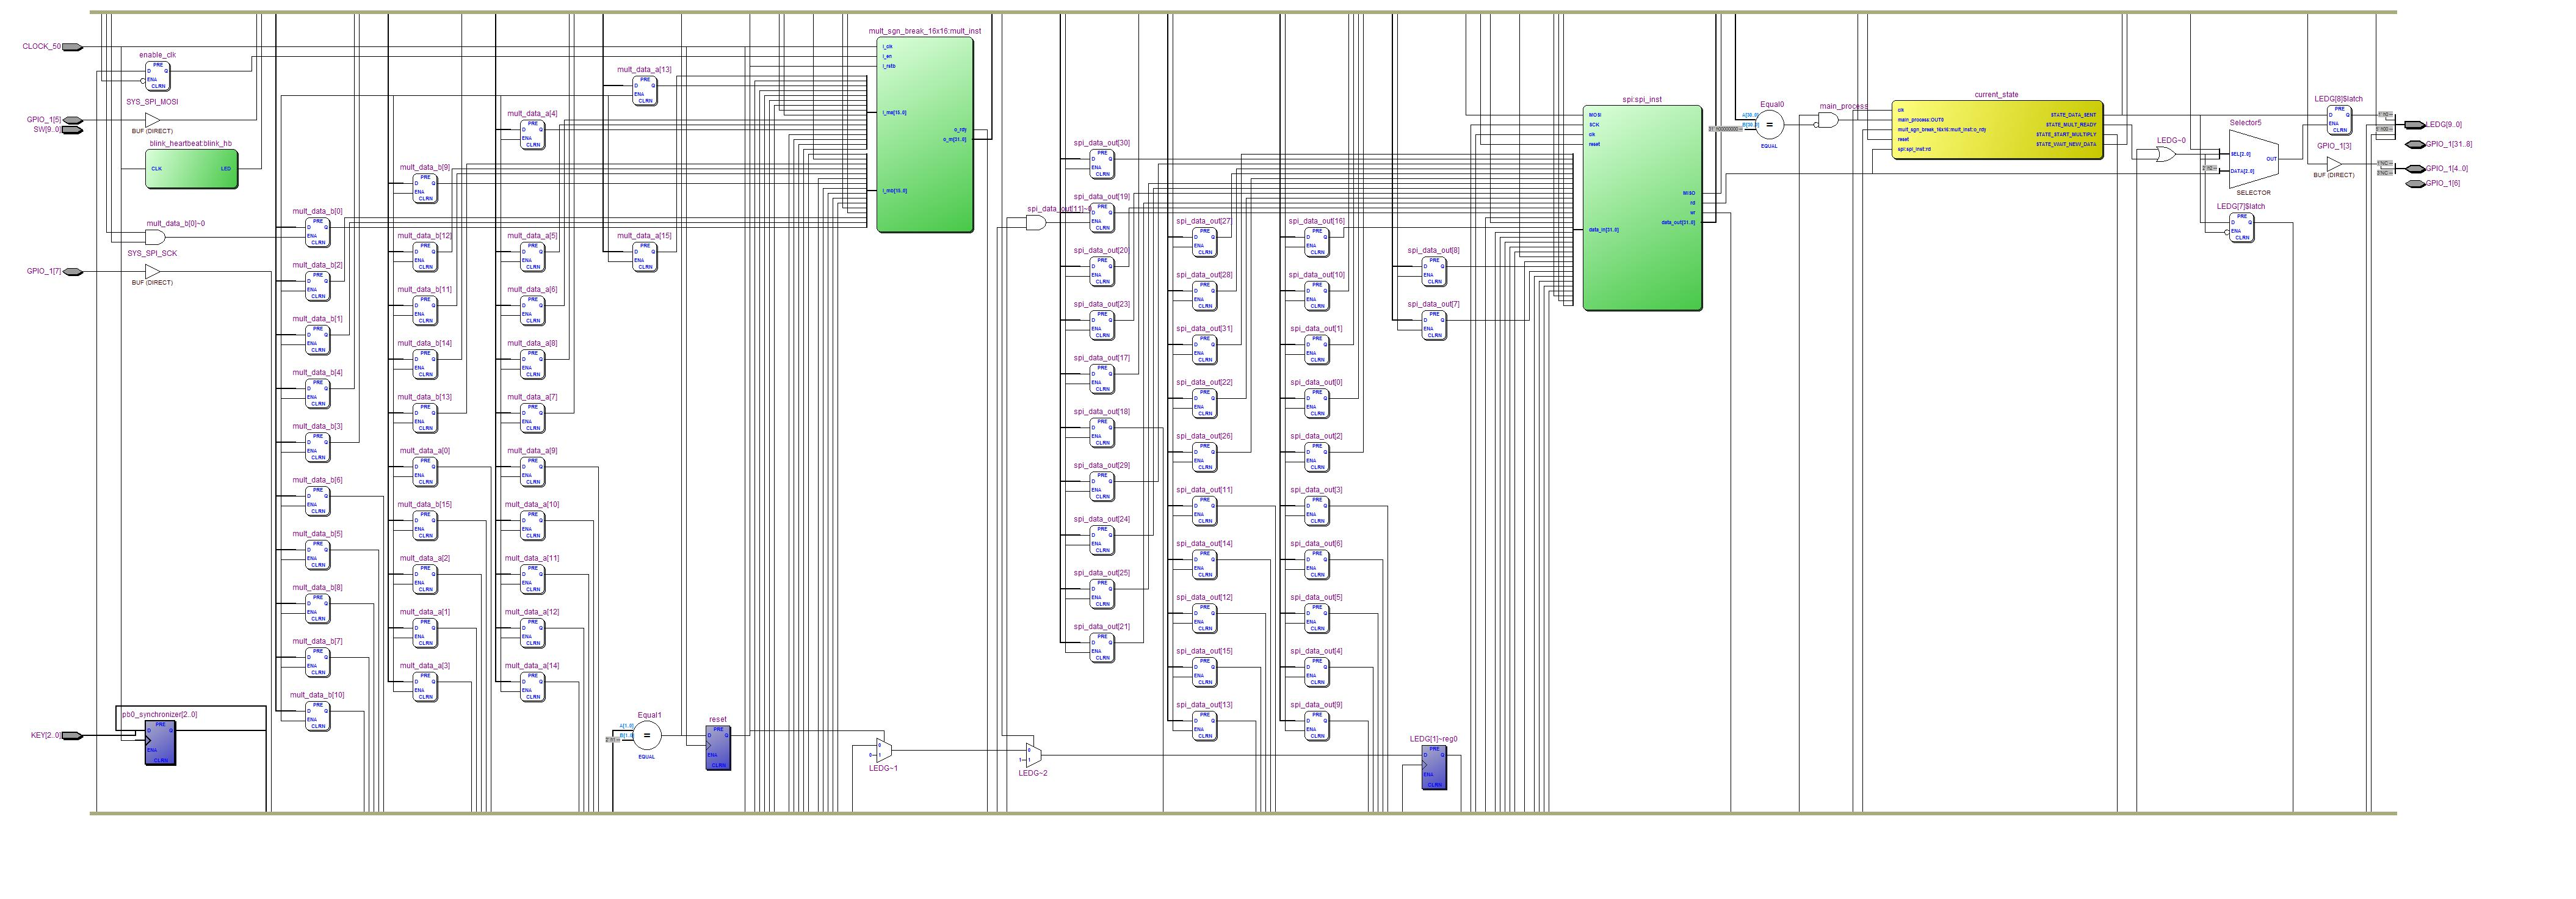
\includegraphics[scale=0.15]{./img/rtl_basic_mult_complete.jpg}
				\caption{Vista RTL integrale ottenuta con \textit{Quartus}}
				\label{fig:rtl_quartus}
			\end{figure}	

			Di seguito uno zoom dell'immagine su alcune parti di interesse: 

			\begin{figure}[H]
				\centering
				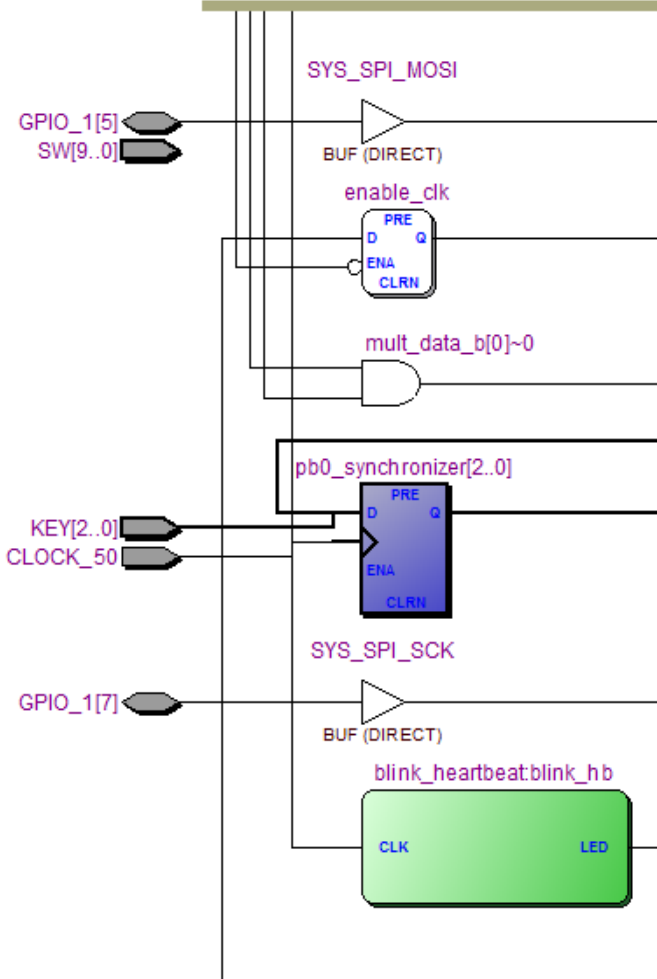
\includegraphics[scale=0.4]{./img/quartus_rtl_viewer_1.png}
				\caption{Prima parte della vista RTL ottenuta con \textit{Quartus}}
				\label{fig:rtl_quartus_1}
			\end{figure}	

			\begin{figure}[H]
				\centering
				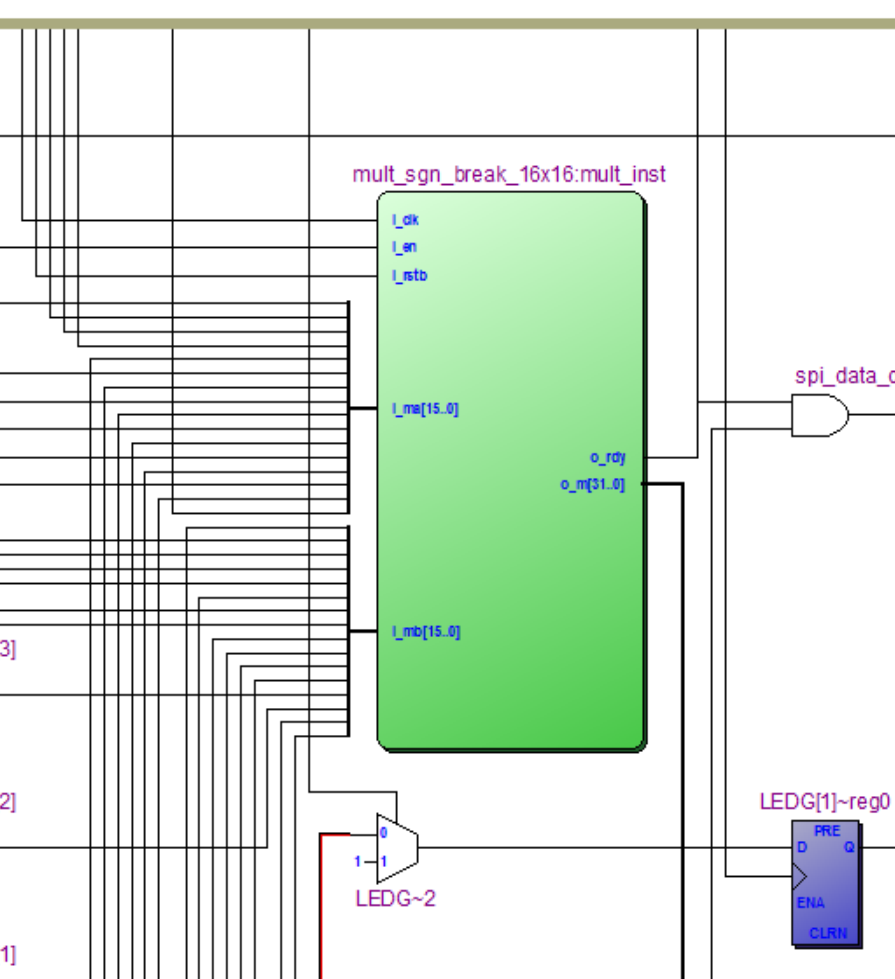
\includegraphics[scale=0.4]{./img/quartus_rtl_viewer_2.png}
				\caption{Seconda parte della vista RTL ottenuta con \textit{Quartus}}
				\label{fig:rtl_quartus_2}
			\end{figure}	

			\begin{figure}[H]
				\centering
				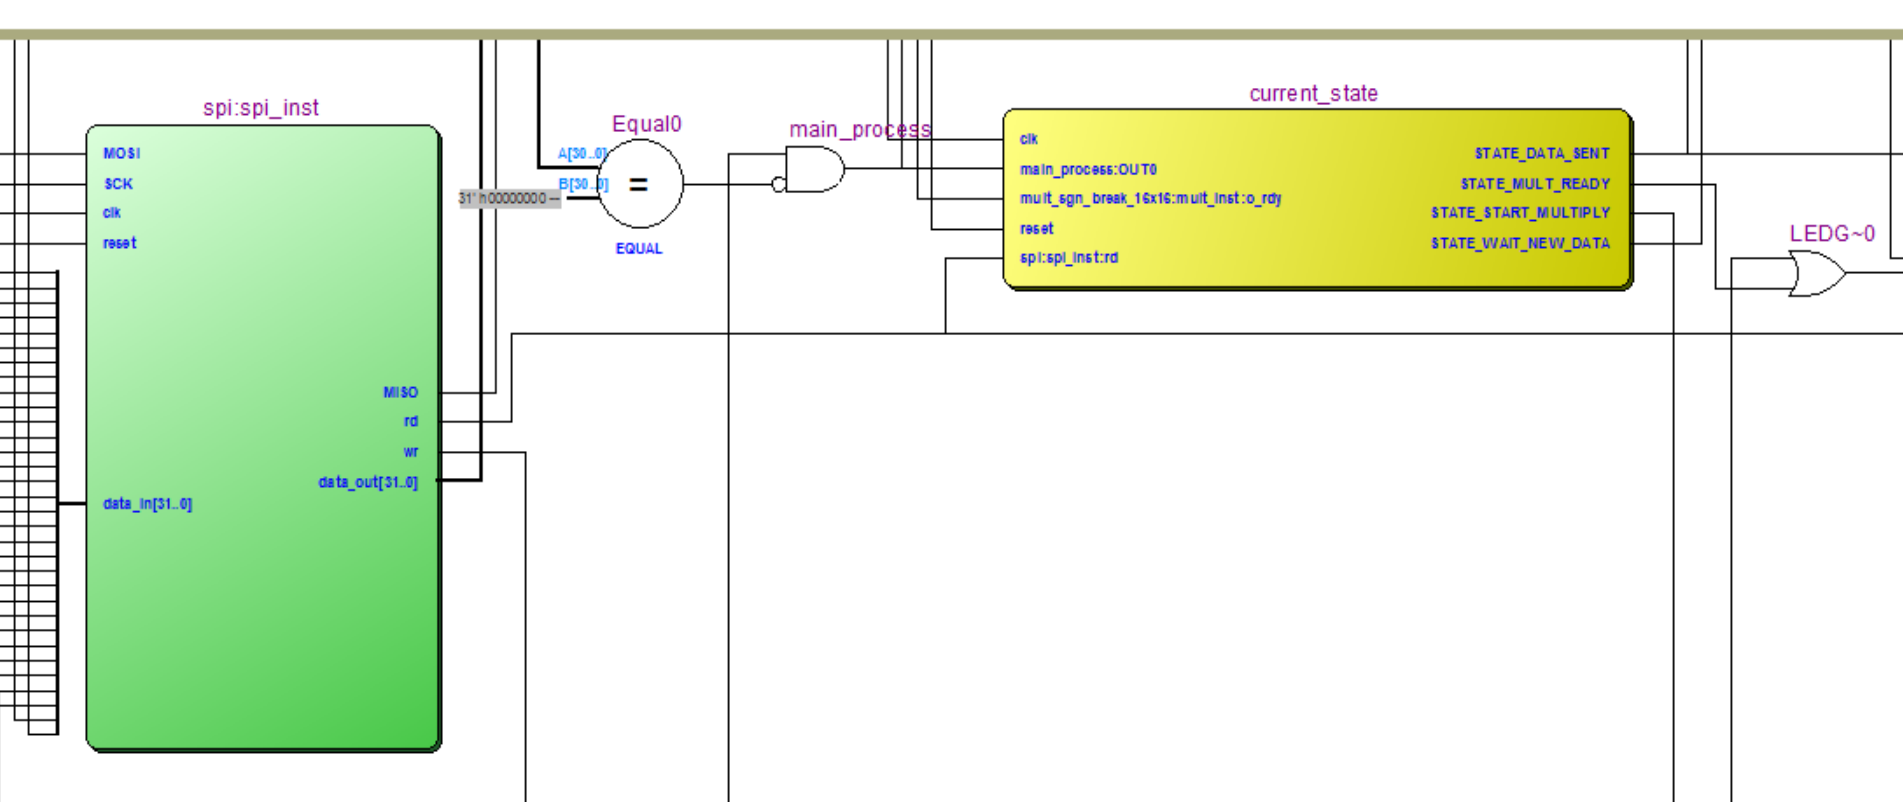
\includegraphics[scale=0.4]{./img/quartus_rtl_viewer_3.png}
				\caption{Terza parte della vista RTL ottenuta con \textit{Quartus}}
				\label{fig:rtl_quartus_3}
			\end{figure}	

			\begin{figure}[H]
				\centering
				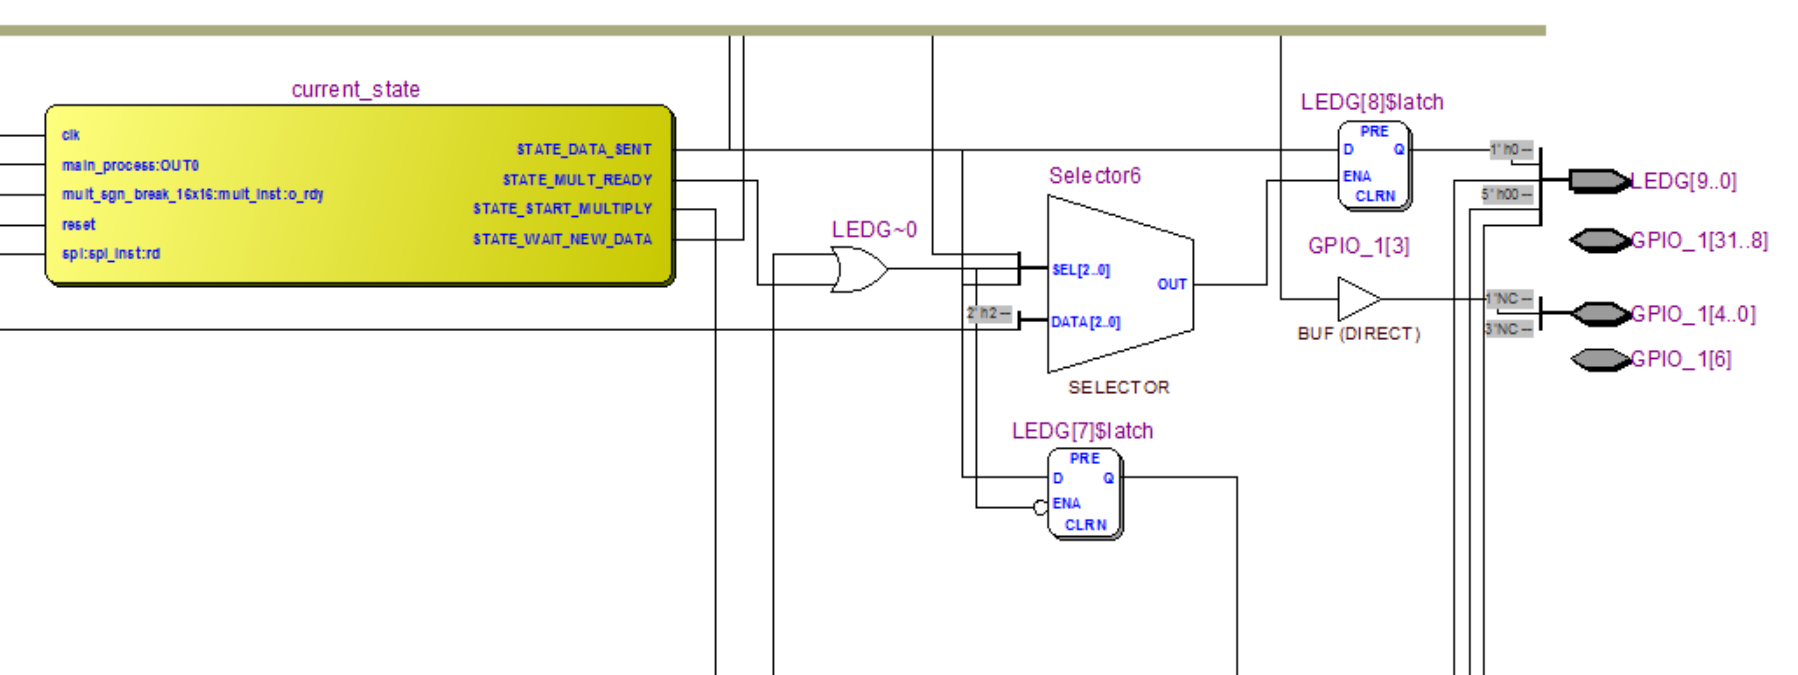
\includegraphics[scale=0.4]{./img/quartus_rtl_viewer_4.png}
				\caption{Quarta parte della vista RTL ottenuta con \textit{Quartus}}
				\label{fig:rtl_quartus_4}
			\end{figure}		

			Salendo di gerarchia, il sistema \textit{basic\_mult} si presenta come \textit{top\_level} dell'architettura.
			La seguente figura mostra la vista del sistema dall'esterno:

			\begin{figure}[H]
				\centering
				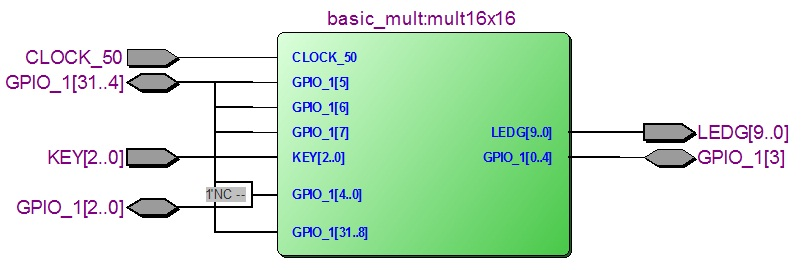
\includegraphics[scale=0.4]{./img/top_basic_mult.jpg}
				\caption{Vista del top level}
				\label{fig:top_level_basic_mult}
			\end{figure}
			
			In particolare, è importante notare che solo \textit{GPIO\_1[3]} è riportato come uscita del sistema poiché, come definito dal file \textit{DE0\_PinAssignment.qpf} fornito durante il corso, corrisponde al \textit{MISO} chè è il pin di output per il dispositivo \textit{SLAVE} nella comunicazione SPI.

	\section*{Modulo SPI}
	\label{subsec:modulo_spi}
	\addcontentsline{toc}{section}{Modulo SPI}
		\subsection*{Fase di implementazione}
		\label{subsec:spi_implementazione}
		\addcontentsline{toc}{subsection}{Fase di implementazione}
			Di seguito viene riportata la vista dell'architettura spi implementata, ottenunta mediante \textit{TerosHDL}.
			
			\begin{figure}[ht]
				\centering
				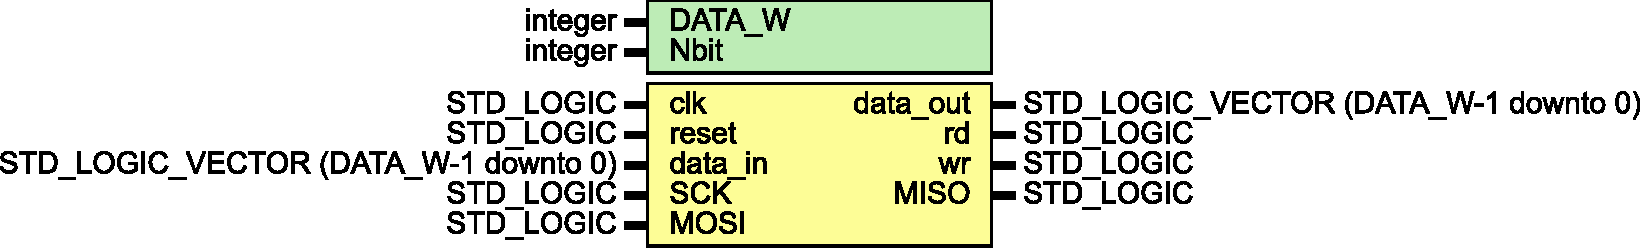
\includegraphics[scale=0.6]{./img/spi_teros.pdf}
				\caption{Architettura modulo spi utilizzato}
				\label{fig:spi_module_teros}
			\end{figure}
			I generic values sono riportati in tabella \ref{tab:spi_generic}.
			\begin{table}[H]
				\begin{tabular}{|l|l|l|p{0.68\textwidth}|}
					\hline
					\textbf{Nome} & \textbf{Tipo} & \textbf{Valore} & \textbf{Descrizione} \\
					\hline
					DATA\_W & integer & 16 & Lunghezza dei dati acquisiti/inviati in bit \\
					Nbit & integer & 4 & $\log_2$(DATA\_W) \\
					\hline
				\end{tabular}
				\caption{Gerneric values per l'architettura SPI implementata}
				\label{tab:spi_generic}
			\end{table}

			In tabella \ref{tab:spi_IO} sono riportati gli input e output dell'architettura.

			\begin{table}[H]
				\centering
				\begin{tabular}{|l|l|p{0.25\textwidth}|p{0.4\textwidth}|}
				\hline
				\textbf{Nome porta} & \textbf{Direzione} & \textbf{Tipo} & \textbf{Descrizione} \\
				\hline
				clk & in & std\_logic & Clock \\
				reset & in & std\_logic & Reset SPI \\
				data\_in & in & std\_logic\_vector (DATA\_W-1 downto 0) & Dati da inviare al master (dimensione DATA\_W-1). \\
				data\_out & out & std\_logic\_vector (DATA\_W-1 downto 0) & Dati letti dal master posti in uscita (dimensione DATA\_W-1). \\
				rd & out & std\_logic & Settato a 1 quando l'operazione di invio in MISO è conclusa. \\
				wr & out & std\_logic & Settato a 1 quando l'operazione di lettura da MOSI è conclusa. \\
				SCK & in & std\_logic & Slave clock \\
				MOSI & in & std\_logic & Master Output Slave Input \\
				MISO & out & std\_logic & Master Input Slave Output \\
				\hline
				\end{tabular}
			\caption{Descrizione degli input/output dell'architettura SPI implementata}
			\label{tab:spi_IO}
			\end{table}
				
			In tabella \ref{tab:spi_signals} sono riportati i segnali implementati nell'architettura.
			\begin{table}[H]
				\begin{tabular}{|l|l|p{0.42\textwidth}|}
					\hline
					\textbf{Segnali} & \textbf{Tipo} & \textbf{Descrizione} \\
					\hline
					spi\_value & std\_logic\_vector(DATA\_W-1 downto 0) & Registro bit da inviare in MISO \\
					spi\_readvalue & std\_logic\_vector(DATA\_W-1 downto 0) & Registro bit letti da MOSI \\
					sck\_synchronizer & std\_logic\_vector(2 downto 0) & Registro per la sincronizzazione con il clock; in particolare è di lunghezza 3 bit dove i bit 2 e 1 permettono l'identificazione della transizione alto-basso o basso-alto del clock SCK. Questo registro viene shiftato a sinistra per ogni colpo di clock e in posizione 0 acquisisce SCK. \\
					rdcnt & unsigned(Nbit-1 downto 0) & Contatore per la fase di lettura di lunghezza Nbit \\
					wrcnt & unsigned(Nbit-1 downto 0) & Contatore per la fase di scrittura di lunghezza Nbit \\
					feed\_me & std\_logic & Se settato a 1, l'operazione di invio in MISO è conclusa e se ne può iniziare un'altra \\
					read\_me & std\_logic & Se settato a 1, l'operazione di acquisizione da MOSI è conclusa e se ne può iniziare un'altra \\
					\hline
				\end{tabular}
				\caption{Segnali dell'architettura SPI implementata}
				\label{tab:spi_signals}
			\end{table}

			Di seguito la descrizione dell'algoritmo implementato che segue la descrizione del mode 1 della	comunicazione SPI:
			\begin{itemize}
				\item Al fronte di salita del clock si shifta a sinistra di una posizione \texttt{sck\_synchronizer} e si pone in \texttt{lsb SCK}.
				\item Se \texttt{reset} è a 1 (attivo) si azzerano i registri \texttt{spi\_value}, \texttt{spi\_readvalue}, \texttt{MISO}, \texttt{rdcnt}, \texttt{wrcnt}, \texttt{rd}, \texttt{wr}, \texttt{read\_me}, \texttt{feed\_me}, \texttt{data\_out}.
				\item Se \texttt{reset} non è 1:
				\begin{itemize}
					\item Se \texttt{sck\_synchronizer(2 downto 1)} è "01" significa che c'è stata una transizione basso-alto, quindi si effettuano le operazioni di trasmissione dei bit:
					\begin{itemize}
						\item Aggiornamento di \texttt{spi\_value} con uno shift a sinistra: \texttt{spi\_value <= spi\_value(DATA\_W-2 downto 0) \& '0'}.
						\item Immissione sulla linea \texttt{MISO} del \texttt{MSB} di \texttt{spi\_value}: \texttt{MISO <= spi\_value(DATA\_W-1)}.
						\item Incremento del contatore dei bit inviati: \texttt{wrcnt <= wrcnt + 1}.
						\item Nel caso in cui il conteggio dei bit inviati sia completato (\texttt{wrcnt = all\_ones}), si effettua l'operazione di azzeramento del contatore: \texttt{wrcnt <= (others => '0')} e si settano a 1 \texttt{feed\_me} e \texttt{rd}: \texttt{feed\_me <= '1'}, \texttt{rd <= '1'}.
					\end{itemize}
					\item Se \texttt{sck\_synchronizer(2 downto 1)} è "10" significa che c'è stata una transizione alto-basso, quindi si effettuano le operazioni di acquisizione:
					\begin{itemize}
						\item Aggiornamento di \texttt{spi\_readvalue} con uno shift a sinistra: \texttt{spi\_readvalue(DATA\_W-1 downto 1) <= spi\_readvalue(DATA\_W-2 downto 0)}.
						\item Lettura del bit sulla linea \texttt{MOSI} e collocamento di esso nel \texttt{LSB} di \texttt{spi\_readvalue}: \texttt{spi\_readvalue(0) <= MOSI}.
						\item Incremento del contatore di bit letti: \texttt{rdcnt <= rdcnt + 1}.
						\item Nel caso in cui il conteggio dei bit letti sia completato (\texttt{rdcnt = all\_ones}), si effettua l'operazione di azzeramento del contatore: \texttt{rdcnt <= (others => '0')} e si settano a 1 \texttt{read\_me} e \texttt{wr}: \texttt{read\_me <= '1'}, \texttt{wr <= '1'}.
					\end{itemize}
					\item Se \texttt{feed\_me} è 1 si aggiorna \texttt{spi\_value} con il nuovo dato da inviare: \texttt{spi\_value <= data\_in} e si mettono a zero i bit relativi a \texttt{rd} e \texttt{feed\_me}: \texttt{rd <= '0'}, \texttt{feed\_me <= '0'}.
					\item Se \texttt{read\_me} è 1 si porta in uscita il dato letto: \texttt{data\_out <= spi\_readvalue} e si mettono a zero i bit relativi a \texttt{read\_me} e \texttt{wr}: \texttt{read\_me <= '0'}, \texttt{wr <= '0'}.
				\end{itemize}
			\end{itemize}

		\subsection*{Fase di sintesi}
		\label{subsec:spi_sintesi}
		\addcontentsline{toc}{subsection}{Fase di sintesi}
			Di seguito viene mostrata la vista RTL dell'entity \texttt{spi\_inst} mostrata nel listato \ref{lst:tb_spi.vhd}.

			\begin{figure}[H]
				\centering
				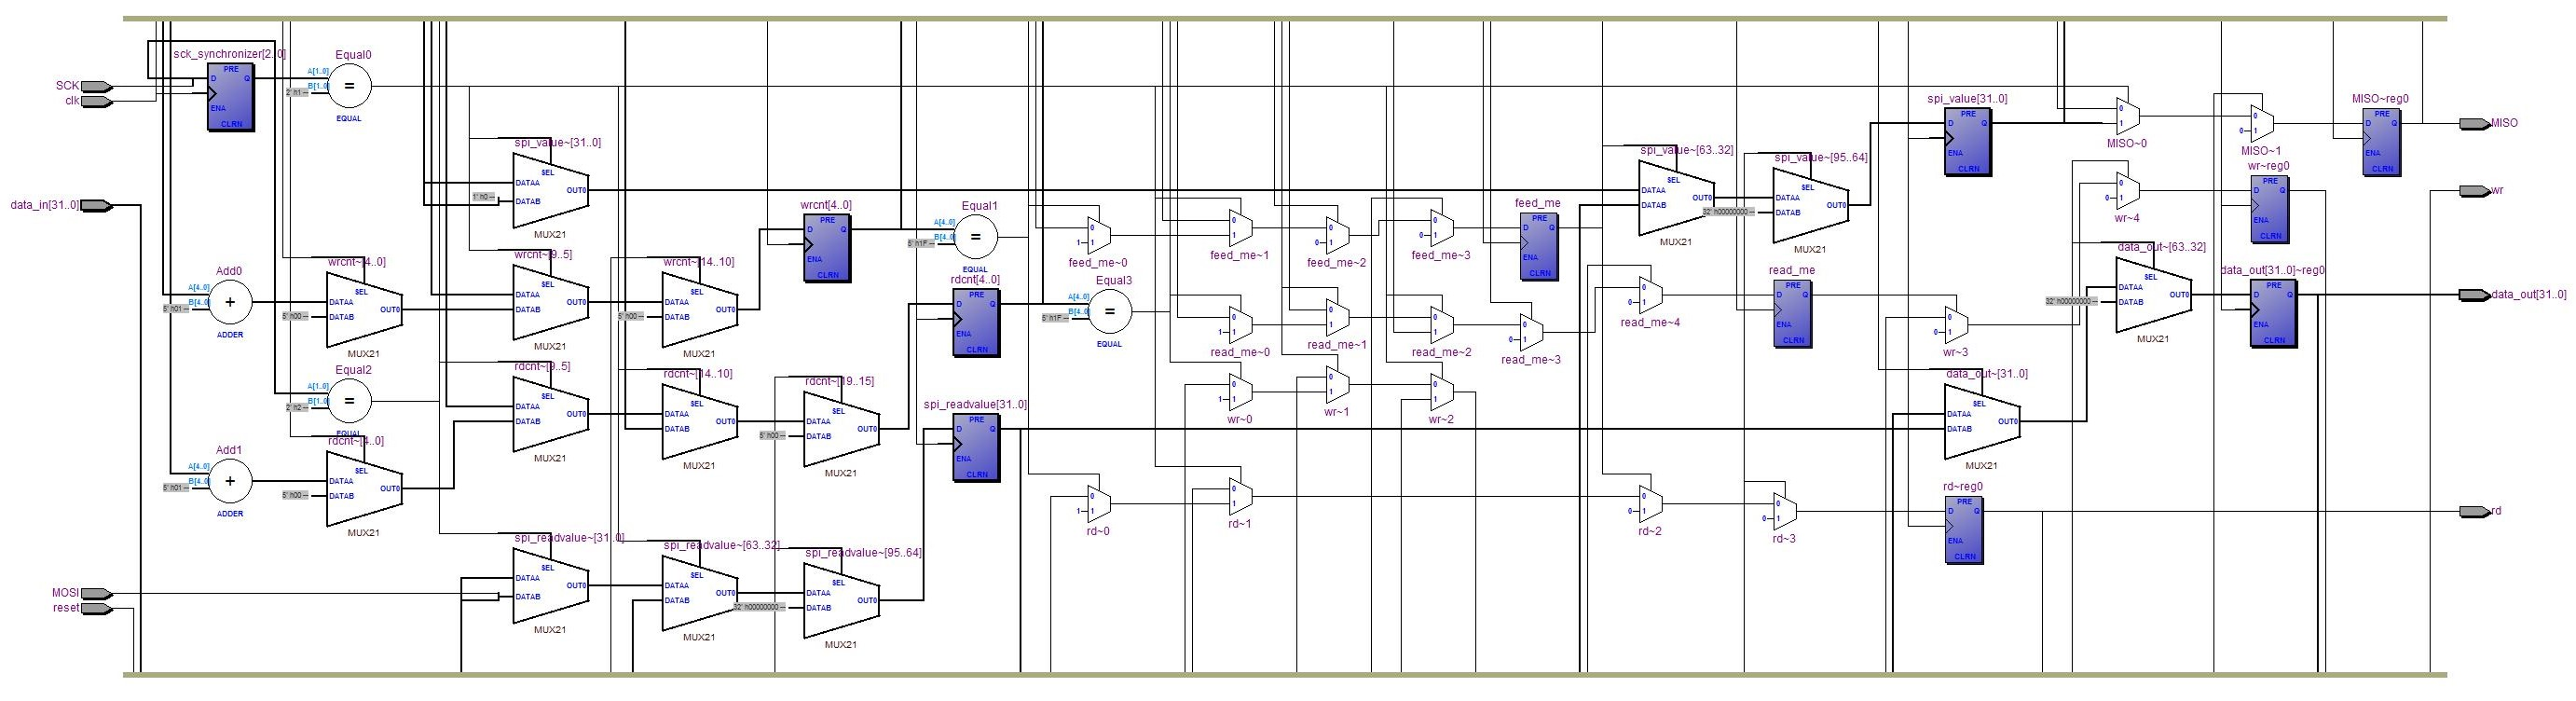
\includegraphics[scale=0.21]{./img/spi_spi_inst.jpg}
				\caption{Vista RTL integrale ottenuta con \textit{Quartus} dell'entity SPI}
				\label{fig:rtl_quartus_spi}
			\end{figure}	
\chapter*{Programmazione di RaspberryPi utilizzando MATLAB Simulink}
\label{ch:programmazione_raspberrypi}
\addcontentsline{toc}{chapter}{Programmazione di RaspberryPi utilizzando MATLAB Simulink}

	\section*{Ruolo di MATLAB Simulink nel progetto}
	\label{sec:ruolo_simulink}
	\addcontentsline{toc}{section}{Ruolo di MATLAB Simulink nel progetto}

		L'integrazione di dispositivi hardware, come il Raspberry Pi, in progetti di ingegneria è un passo cruciale per realizzare soluzioni complesse e interconnesse. Una delle metodologie di programmazione che si è dimostrata efficace e versatile è l'uso del tool "Hardware for RaspberryPi" di MATLAB Simulink.

		"Hardware for RaspberryPi" è un potente strumento che permette di creare applicazioni personalizzate per il Raspberry Pi in modo grafico. Sfruttando l'approccio a blocchi di Simulink, è possibile progettare e sviluppare in modo rapido algoritmi, controlli e interfacce utente che possono essere implementati direttamente sul Raspberry Pi. Questo tool offre una vasta libreria di blocchi funzionali come il controllo di GPIO, comunicazione con sensori, attuatori e dispositivi esterni. 
		
		Un aspetto particolarmente vantaggioso dell'utilizzo di "Hardware for RaspberryPi" è la sua capacità di generare automaticamente il codice C++ ottimizzato per il Raspberry Pi. Ciò significa che dopo aver creato il modello in Simulink, è possibile generare il codice e caricarlo direttamente sul Raspberry Pi, semplificando il processo di deploy e testing.
		
		È importante notare che "Hardware for RaspberryPi" non è compatibile con le versioni di MATLAB 2022a e successive. È stato testato con successo su MATLAB 2017b, ma non è stato valutato per versioni intermedie tra 2017b e 2022a. Nonostante non sembri esserci alcun problema di compatibilità con la versione di MATLAB, poiché il tool si installa correttamente, esso non compila il blocco simulink creato.

		In questo progetto, si è utilizzato il tool "Hardware for RaspberryPi" per gestire la comunicazione SPI come master, impiegando il blocco "SPI Master Transfer". Questa scelta si è rivelata essenziale per coordinare in modo efficiente la comunicazione tra l'FPGA e il Raspberry Pi, permettendo lo scambio di dati e il controllo dei segnali nel contesto del progetto in corso.

		\begin{figure}[ht]
			\centering
			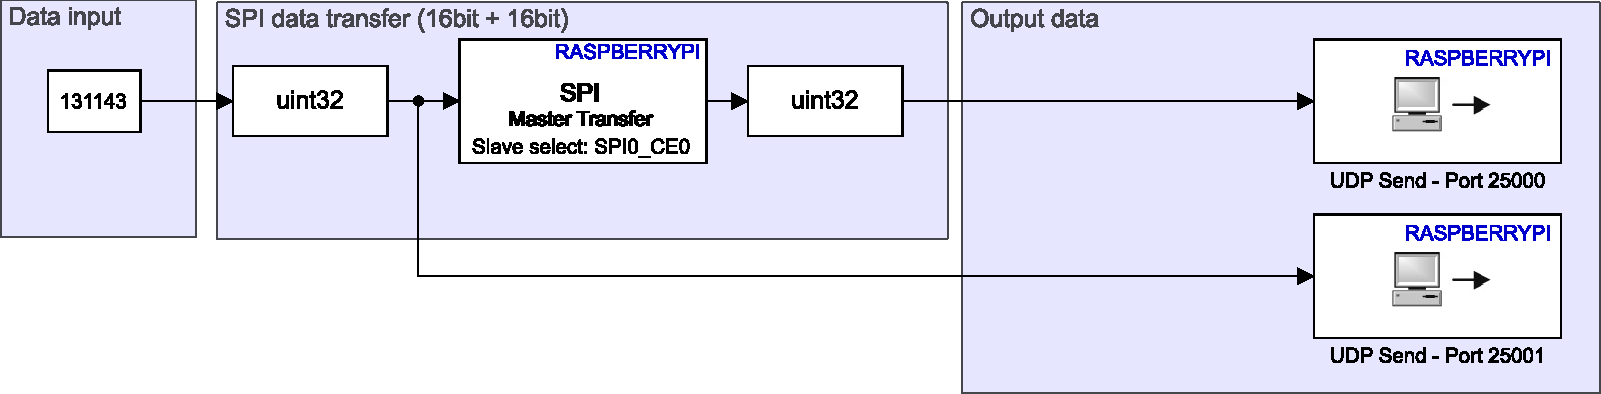
\includegraphics[scale=0.6]{./img/test_raspi_psed_single.pdf}
			\caption{Schema a blocchi simulink implementato}
			\label{fig:simulink_sch}
		\end{figure}

		Lo schema mostrato in figura \ref{fig:simulink_sch} mostra il funzionamento della comunicazione SPI su RaspberryPi. Esso invia periodicamente il numero $131143$ che è l'unione di due numeri a 16 bit, (0x02 $<<$ 16) $\mid$ 0x47 (corrispondenti ai numeri 2 e 71 in base 10), che saranno il moltiplicando e il moltiplicatore della moltiplicazione che dovrà eseguire l'FPGA. Il risultato poi verrà ritornato da FPGA e sarà un numero a 32 bit, di valore atteso 142 ossia 0x8E.

		I valori che vengono letti in ingresso al raspberry verranno poi inviati su seriale ethernet utilizzando il protocollo UDP.

	\section*{Configurazione e comunicazione con Raspberry Pi}
	\label{sec:configurazione_raspberrypi}
	\addcontentsline{toc}{section}{Configurazione e comunicazione con RaspberryPi}
			
		Per la creazione di un canale di comunicazione tra \textit{RaspberryPi} e la FPGA \textit{Cyclone III} si è utilizzato il protocollo di comunicazione SPI.

		Di seguito vengono esposti nella tabella \ref{tab:wiring} i collegamenti da effettuare sulle due board, visualizzabili in figura \ref{fig:wiring}:

		\begin{table}[ht]
			\centering
			\begin{tabular}{|l|l|}
				\rowcolor{gray!25} % Imposta il colore di sfondo della riga
				\hline
				\textbf{FPGA} & \textbf{Raspberry} \\
				\hline
				GPIO1\_D1 & GPIO8 (CE0) \\
				\hline
				GPIO1\_D3 & GPIO9 (MISO) \\
				\hline
				GPIO1\_D5 & GPIO10 (MOSI) \\
				\hline
				GPIO1\_D7 & GPIO11 (SCK) \\
				\hline
			\end{tabular}
			\caption{Collegamenti pin to pin delle due board}
			\label{tab:wiring}
		\end{table}

		\begin{figure}[ht]
			\centering
			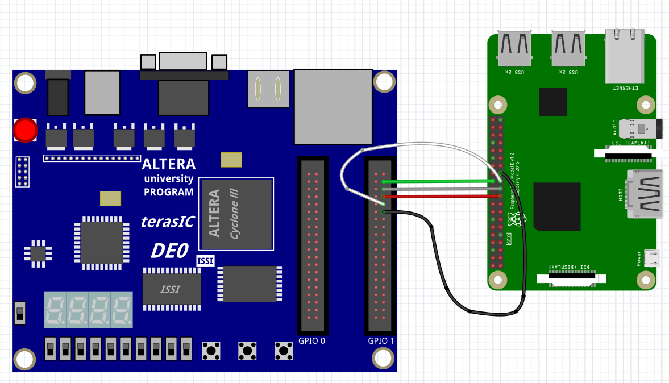
\includegraphics[scale=0.6]{./img/link_fpga_raspi.png}
			\caption{Schema di collegamento visivo tra le due schede}
			\label{fig:wiring}
		\end{figure}

		\subsection*{Funzionamento della Comunicazione SPI}
		\label{subsec:funzionamento_spi_comm}
		\addcontentsline{toc}{subsection}{Funzionamento della comunicazione SPI}
			La comunicazione SPI (\textit{Serial Peripheral Interface}) è un protocollo di comunicazione seriale ampiamente utilizzato nell'ambito dell'elettronica embedded. È utilizzato per collegare dispositivi digitali tra loro, consentendo loro di scambiare dati in modo sincrono e affidabile. 

			Il funzionamento della comunicazione SPI si basa su una connessione di tipo master-slave tra dispositivi. In questa configurazione, un dispositivo agisce da "master" e controlla il flusso dei dati, mentre uno o più dispositivi agiscono da "slave" e rispondono alle richieste del master. Il master è responsabile di generare il segnale di clock (SCK) che sincronizza la trasmissione e ricezione dei dati.

			I segnali chiave utilizzati nella comunicazione SPI sono:
			\begin{itemize}
			\item \textbf{SCK (\textit{Serial Clock}):} Questo segnale viene generato dal master e utilizzato per sincronizzare la trasmissione e ricezione dei dati tra i dispositivi. I dati vengono campionati sul fronte di salita o discesa del segnale di clock, a seconda della configurazione.
			
			\item \textbf{MOSI (\textit{Master Output Slave Input}):} Questo è il segnale di uscita del master e di ingresso dello slave. Il master utilizza MOSI per inviare dati agli slave. Quando i dati vengono trasmessi, vengono spostati bit per bit lungo il MOSI, sincronizzati dal segnale di clock.
			
			\item \textbf{MISO (\textit{Master Input Slave Output}):} Questo è il segnale di ingresso del master e di uscita dello slave. Gli slave utilizzano MISO per inviare dati al master. Anche in questo caso, i dati vengono spostati bit per bit lungo il MISO, sincronizzati dal segnale di clock.
			
			\item \textbf{SS/CS (\textit{Slave Select/Chip Select}):} Questo segnale è utilizzato per selezionare uno specifico slave con cui il master vuole comunicare. Il master può avere più linee SS/CS per comunicare con diversi slave. Nel nostro caso indicato come CE0, ovvero \textit{chip enable 0}
			\end{itemize}

			Il funzionamento di una trasmissione SPI inizia quando il master seleziona uno specifico slave mediante il segnale SS/CS. Successivamente, il master inizia a inviare i dati lungo il MOSI, sincronizzati dal segnale di clock SCK. Gli slave campionano i dati in arrivo sul fronte di salita o discesa del segnale di clock e li trasmettono al master tramite il segnale MISO.

			La comunicazione SPI può funzionare sia in modalità full-duplex, in cui il master e lo slave possono trasmettere contemporaneamente, che in modalità half-duplex, in cui la trasmissione avviene in entrambe le direzioni, ma non contemporaneamente.

			\begin{figure}[ht]
				\centering
				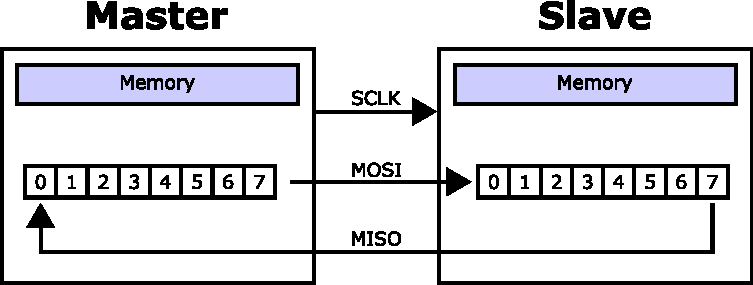
\includegraphics[scale=0.5]{./img/SPI_8-bit_circular_transfer.pdf}
				\caption{Esempio di comunicazione spi}
				\label{fig:spi_example_comm}
			\end{figure}

			Il master deve anche configurare polarità (CPOL) e fase (CPHA) del clock SCK. A seconda dei valori di CPOL e CPHA si distinguono 4 modalità di comunicazione SPI.


			\begin{figure}[ht]
				\centering
				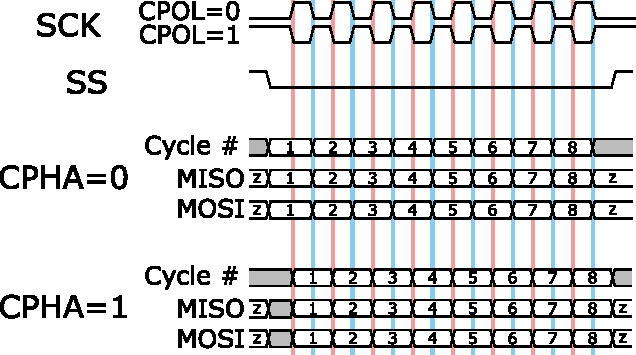
\includegraphics[scale=0.75]{./img/SPI_timing_diagram.pdf}
				\caption{Diagramma temporale delle modalità di comunicazione SPI}
				\label{fig:spi_timing}
			\end{figure}

			\begin{itemize}
			  \item CPOL=0: Il valore base del clock SCK è '0' (lo stato active è 1 e lo stato idle è 0).
				\begin{itemize}
				  \item CPHA=0: acquisizione sul fronte di salita del clock, invio sul fronte di discesa.
				  \item CPHA=1: acquisizione sul fronte di discesa del clock, invio sul fronte di salita.
				\end{itemize}
			  \item CPOL=1: Il valore base del clock SCK è '1' (lo stato active è 0 e lo stato idle è 1).
				\begin{itemize}
				  \item CPHA=0: acquisizione sul fronte di discesa del clock, invio sul fronte di salita.
				  \item CPHA=1: acquisizione sul fronte di salita del clock, invio sul fronte di discesa.
				\end{itemize}
			\end{itemize}
			
			La modalità implementata è: CPOL=0, CPHA=1.

\chapter*{Visualizzazione del dato in rete}
\label{ch:visualizzazione_udp}
\addcontentsline{toc}{chapter}{Visualizzazione del dato in rete}
	L'implementazione di una comunicazione affidabile e veloce è diventata cruciale in molte applicazioni moderne, spaziando dall'Internet delle Cose (IoT) al controllo industriale. In questo contesto, è emerso un tool fondamentale: il protocollo User Datagram Protocol (UDP) su Ethernet. Questo protocollo permette di trasmettere dati in modo efficiente attraverso reti locali senza l'onere di una connessione stabilita.

	Per abbracciare questa metodologia, è stato creato uno script personalizzato in linguaggio Python, attingendo al suo potenziale nel mondo dell'automazione e delle reti. Questo script è stato progettato per consentire la visualizzazione fluida dei dati attraverso la comunicazione UDP su Ethernet

	Per creare lo script, ho sfruttato la flessibilità e la semplicità di Python per gestire la comunicazione UDP. Ho utilizzato la libreria socket di Python per creare un socket UDP e stabilire un canale di comunicazione tra il mittente e il destinatario. Successivamente, ho implementato il formato di trasmissione dei dati e il meccanismo di ricezione per garantire che i dati vengano correttamente incapsulati e decodificati all'altro capo.

	Una caratteristica chiave dello script è la sua adattabilità. Il codice è stato scritto in modo che sia possibile specificare l'indirizzo IP e la porta del destinatario, consentendo la configurazione flessibile della comunicazione tra i dispositivi all'interno della rete. Questa caratteristica permette di integrare lo script in una varietà di contesti e scenari, dalla visualizzazione dei dati a scopi di monitoraggio all'integrazione con applicazioni di controllo.

	Va notato che l'utilizzo di questo protocollo è particolarmente adatto per reti locali, ma potrebbe non essere adatto per scenari in cui l'affidabilità della comunicazione è critica, data la sua natura non garantita e la mancanza di conferme di ricezione. Inoltre, è importante sottolineare che lo script è stato creato e testato con successo su versioni di Python anteriori alla 3.10. \par

	Di seguito viene riportato il codice python utilizzato per la lettura dei dati inviati da RaspbberryPi:

	\begin{lstlisting}[label={lst:udp_listener.py},caption={Script \texttt{udp\_listener.py} per l'ascolto della porta UDP utilizzata dal RaspberryPi}, language=python]
import socket

def main():
	# Creazione di un socket UDP
	udp_socket = socket.socket(socket.AF_INET, socket.SOCK_DGRAM)

	# Selezione di IP e numero di porta da ascoltare
	ip_address = '0.0.0.0'  # Ascolta su tutte le interfacce disponibili
	port = 25000

	# Associazione del socket all'indirizzo IP e alla porta
	udp_socket.bind((ip_address, port))

	# Feedback di avvio
	print(f"Ascolto UDP avviato su {ip_address}:{port}")

	# Main loop
	while True:
		# Ricezione di dati e IP del mittente
		data, address = udp_socket.recvfrom(1024)

		# Verifica su dati non vuoti prima di stamparli
		if data and data != b'\x00' * len(data):
			print(f"Ricevuti {len(data)} byte da {address[0]}:{address[1]}")
			print(f"Dati ricevuti (RAW): {data.hex()}")  # Stampa dei dati in formato esadecimale (hex)

if __name__ == '__main__':
    main()
	\end{lstlisting}

	Di seguito viene mostrato l'output prodotto dallo script Python in ascolto al socket UDP.

	\begin{figure}[H]
		\centering
		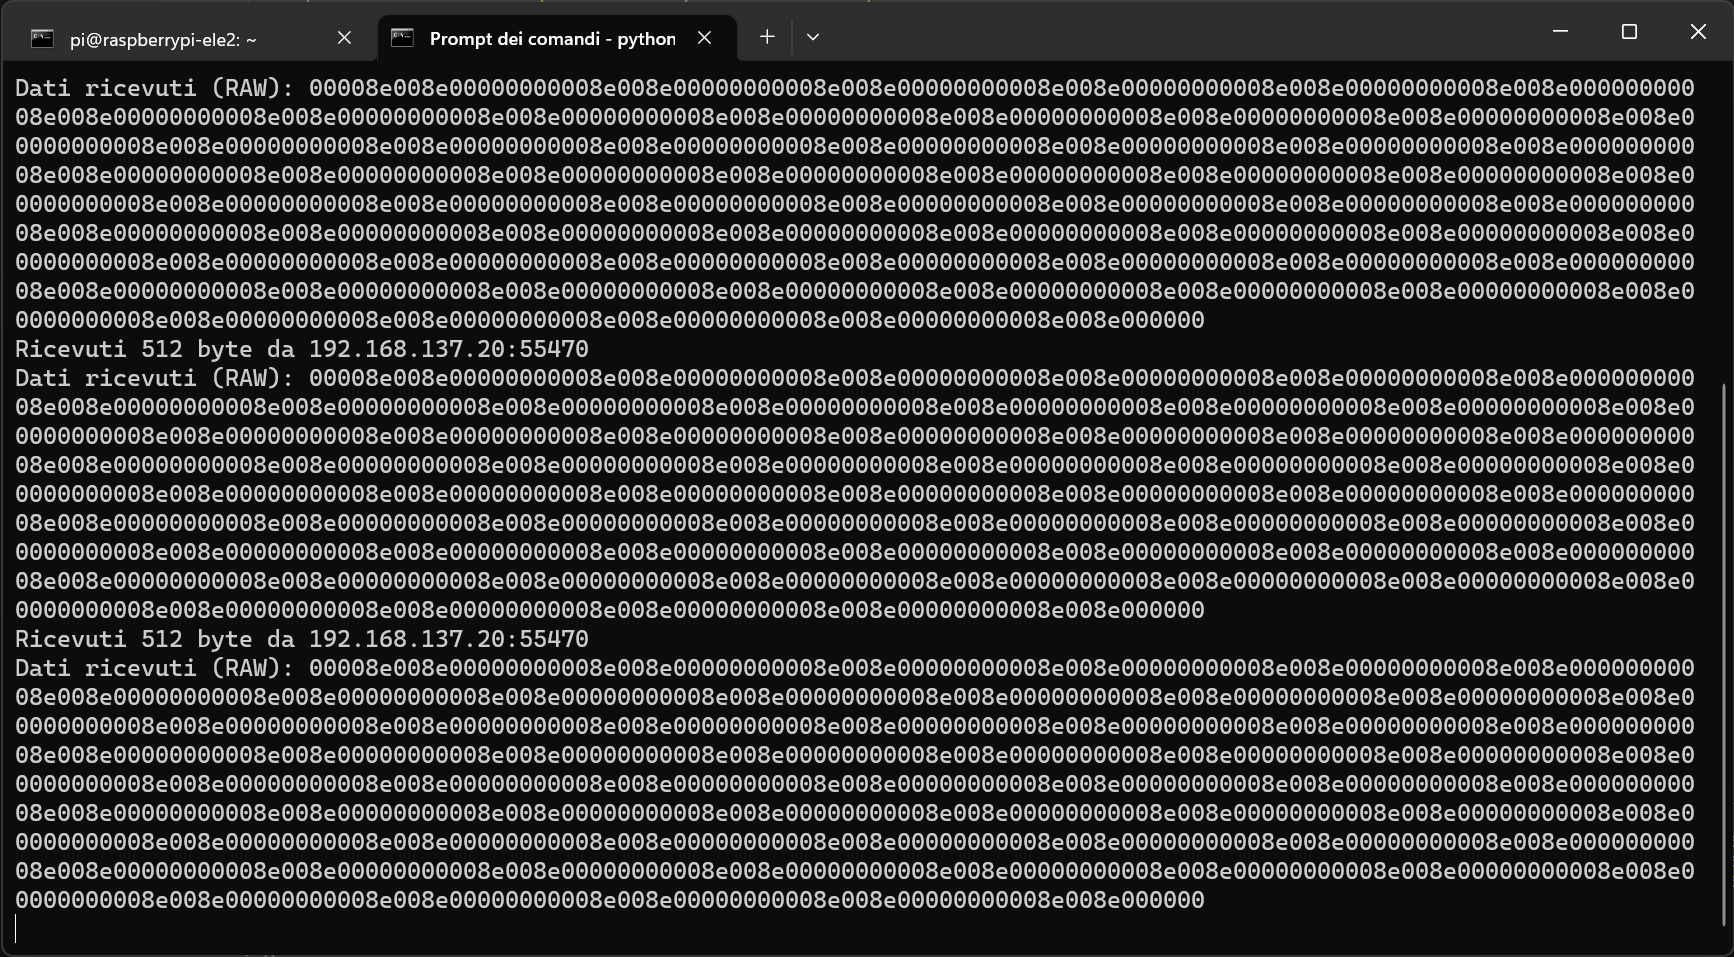
\includegraphics[scale=0.55]{./img/output_python.png}
		\caption{\textbf{udp\_listener.py} - Output dello script python}
		\label{fig:udp_listener_output}
	\end{figure}
	
\chapter*{Risultati sperimentali}
\label{ch:risultati_sperimentali}
\addcontentsline{toc}{chapter}{Risultati sperimentali}

	\section*{Studio comportamentale}
	\label{sec:studio_comportamentale}
	\addcontentsline{toc}{section}{Studio comportamentale}
		La simulazione è stata effettuata utilizzando il software \textit{Altera Modelsim} e, in particolare, il file \texttt{tb\_spi.vhd} esposto nel listato \ref{lst:tb_spi.vhd}.
		La figura \ref*{fig:modelsim_sim_completa}, presenta la simulazione completa di tutti gli stati del sistema.

		\begin{figure}[H]
			\centering
			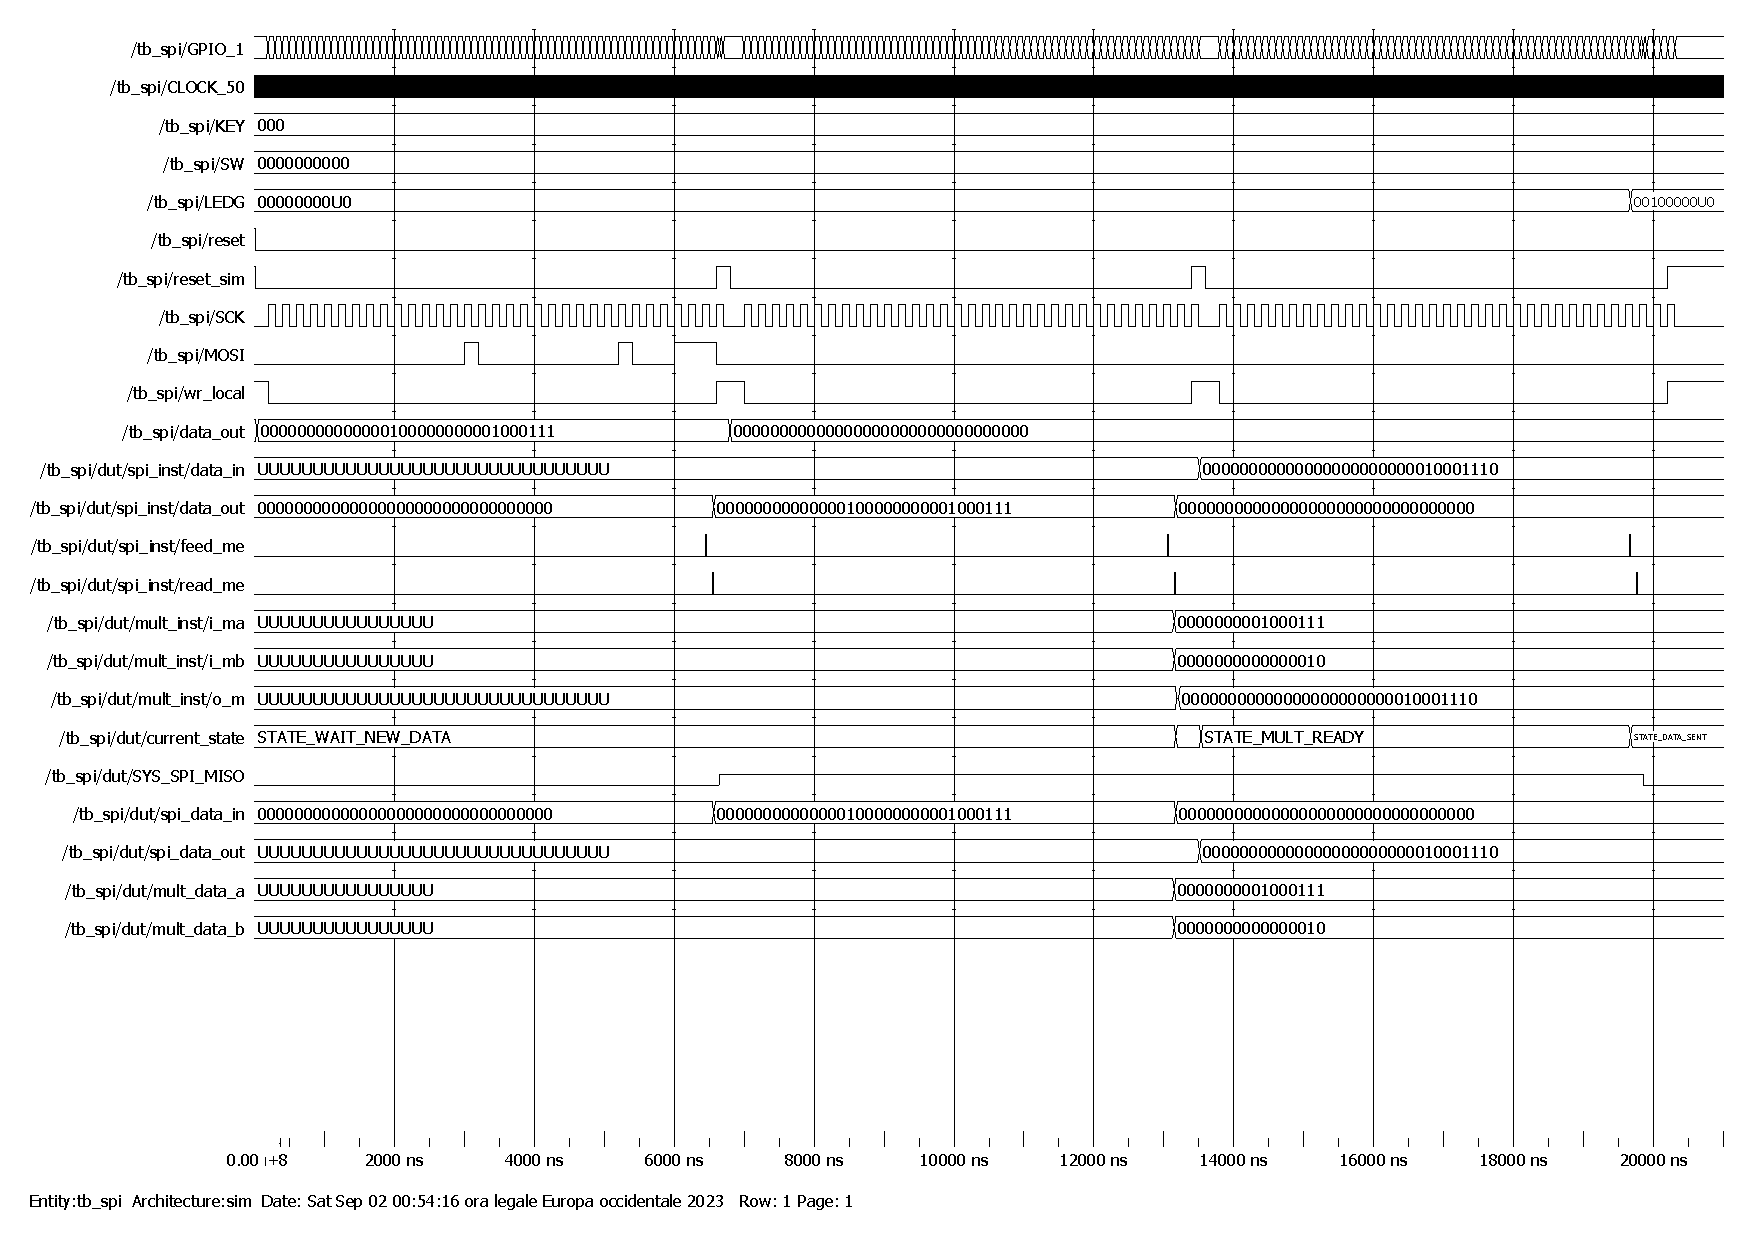
\includegraphics[scale=0.5]{./img/simulation.pdf}
			\caption{Simulazione completa ottenuta con Modelsim}
			\label{fig:modelsim_sim_completa}
		\end{figure}

		In dettaglio, vengono esposti tutti i \texttt{signal} coinvolti nel processo di moltiplicazione e invio del dato. Infatti, si è simulato l'invio e la ricezione del dato come se fossero stati ottenuti mediante una comunicazione SPI.

		Sempre in riferimento al listato \ref*{lst:tb_spi.vhd}, il periodo di clock dell'FPGA, denominato \texttt{clk\_period}, e il periodo di clock di comunicazione SPI, denominato \texttt{sck\_period}, sono due valori costanti che definiscono i tempi operativi di lavoro. Ovviamente, il periodo di comunicazione deve necessariamente essere maggiore del periodo di lavoro: per la simulazione si è scelto un periodo di clock di 20ns mentre il periodo di comunicazione è stato impostato a 200ns.

		Con questi valori operativi, la simulazione mostrata in figura \ref{fig:modelsim_sim_completa} riporta un tempo di circa 2ms da quando il dato viene inviato su SPI prima che ritorni il dato moltiplicato al Raspberry Pi.

		È importante notare che lo stato \texttt{STATE\_WAIT\_NEW\_DATA} permane nonostante il dato sia già presente. Questo è dovuto al controllo che viene effettuato all'interno della macchina a stati. Con riferimento al listato \ref*{lst:mul16_process}, in particolare alla riga \texttt{108}, il controllo per il passaggio di stato vuole che sia presente il flag \texttt{newdata} (collegato al signal \texttt{feed\_me} dell'entity SPI) e che il signal \texttt{spi\_data\_in} sia diverso da 0.  Tuttavia, poiché il signal \texttt{feed\_me} si aggiorna sul fronte di discesa del clock di comunicazione \texttt{SCK} mentre il segnale \texttt{data\_out} si aggiorna sul fronte di salita successivo del clock di comunicazione. Non avendo il processo \texttt{main\_process} nella sua \textit{sensitivity list} il signal \texttt{spi\_data\_in}, la macchina a stati si aggiorna al signal \texttt{feed\_me} successivo.
		Questa può essere considerata un imprecisione dell'architettura ma non ne compromette il funzionamento.

		Alla conferma di ricezione del dato, esso viene scomposto nei due operandi e viene effettuato il passaggio di stato della macchina a stati nello stato \texttt{STATE\_START\_MULTIPLY}. Nella figura \ref{fig:modelsim_sim_completa} queste operazioni sono visibili nei signal \texttt{mult\_data\_a} e \texttt{mult\_data\_b} che passano da una condizione \texttt{UNDEFINED} ad un valore determinato, in particolare ai numeri \texttt{2} e \texttt{71} presentati in notazione binaria.

		Successivamente, al termine delle operazioni di moltiplicazione, lo stato passa al valore \texttt{STATE\_MULT\_READY} indice della presenza del dato correttamente moltiplicato e pronto per essere inviato su seriale SPI. È possibile visualizzare il risultato della moltiplicazione in prossimità dello stato corrispondente osservando il signal \texttt{o\_m} oppure il signal \texttt{dut:spi\_data\_out}.

		Infine, al termine dell'invio del dato il sistema passa allo stato \texttt{STATE\_DATA\_SENT} terminando così il suo ciclo operativo, in attesa di un nuovo segnale di reset per ripartire. In questo caso, non è stato possibile visualizzare in simulazione il corretto movimento del signal \texttt{MISO} per problemi di architettura e direzione dei port.
		Tuttavia, il risultato ottenuto è in linea con i risultati ottenuti per la ricezione del dato in ingresso quindi è possibile sostenere che il tempo impiegato dal sistema al passaggio di stato tra lo stato \texttt{STATE\_MULT\_READY} e lo stato \texttt{STATE\_DATA\_SENT} sia un tempo congruo per l'invio di un dato di 32bit su seriale SPI con periodo di clock SCK di 200ns.

	\section*{Analisi temporale}
	\label{sec:Analisi_Temporale}
	\addcontentsline{toc}{section}{Analisi temporale}
		\begin{figure}[H]
			\centering
			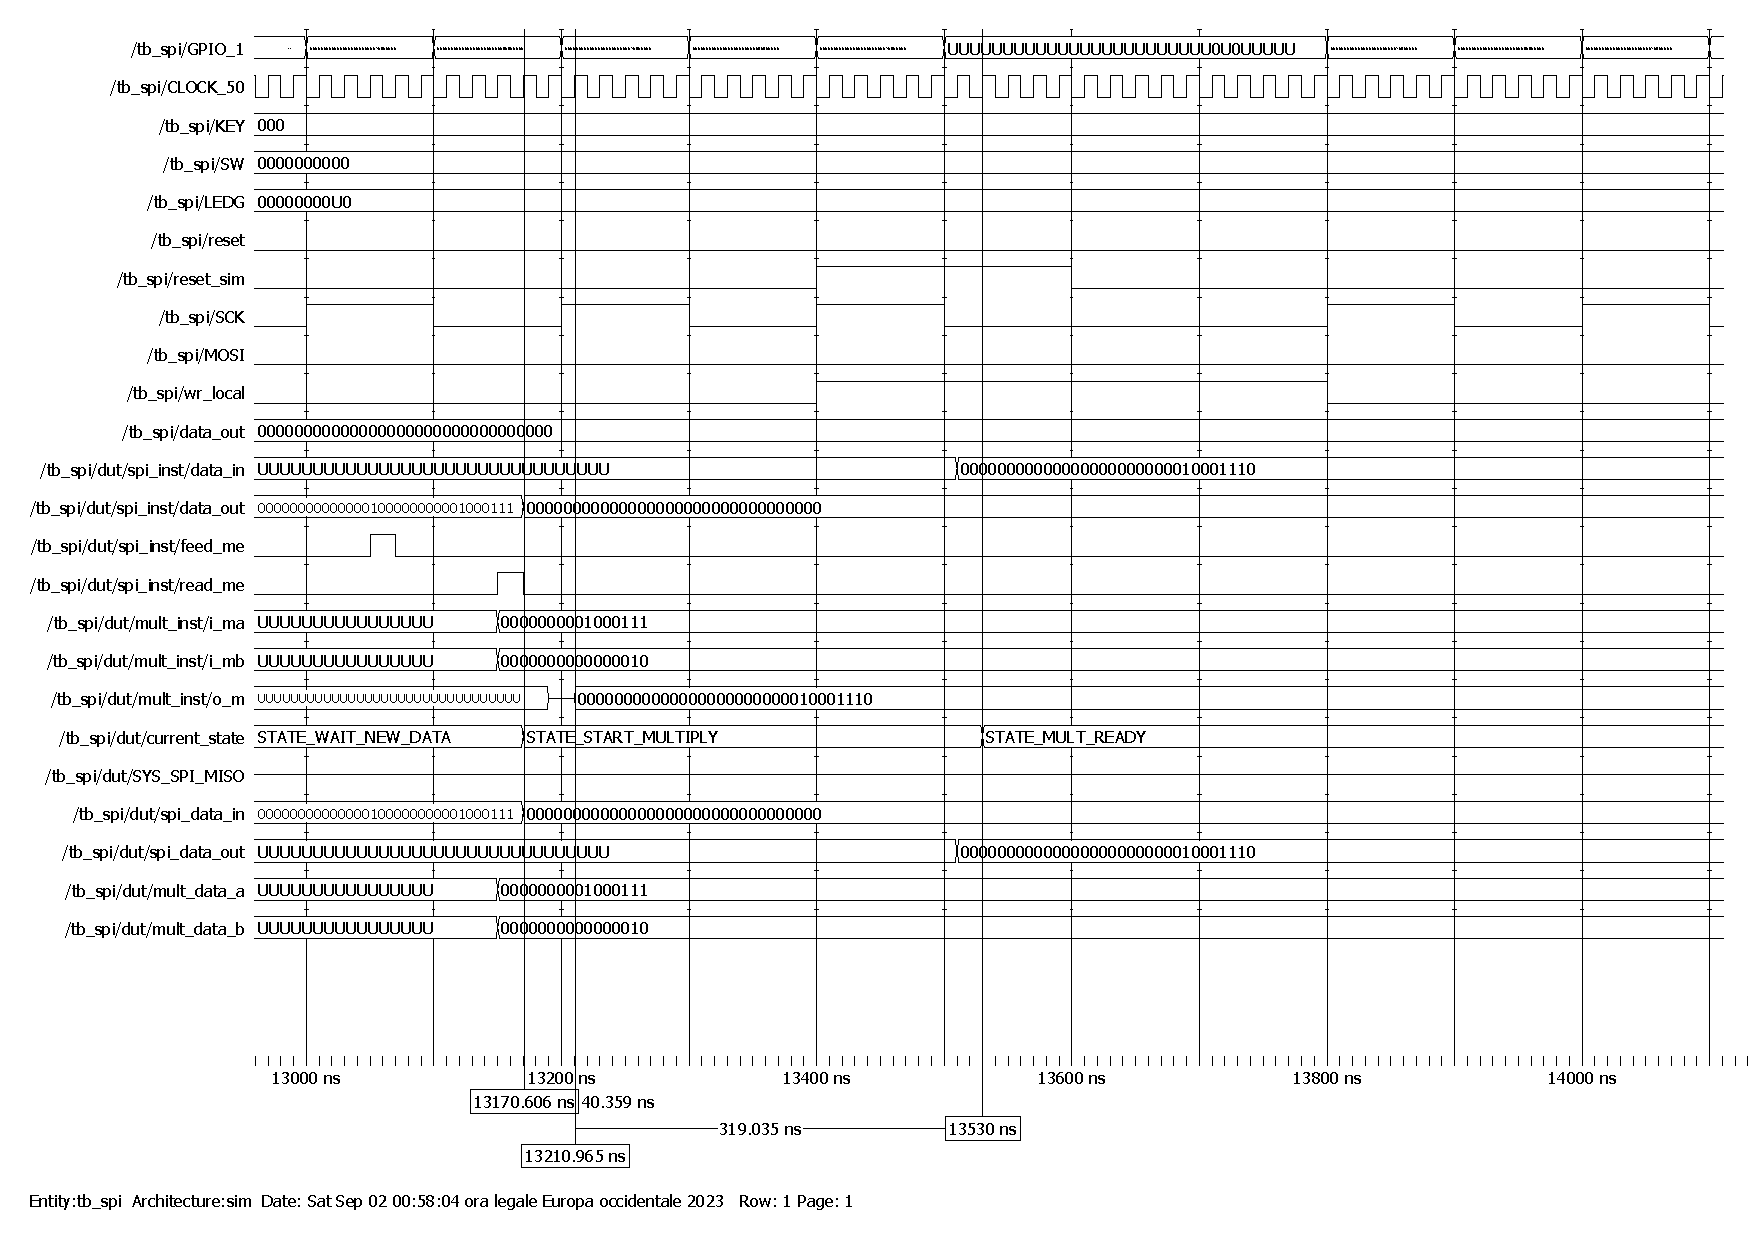
\includegraphics[scale=0.5]{./img/sim_zoom_mult.pdf}
			\caption{Focus della simulazione ottenuta con Modelsim sullo stato di avvio della moltiplicazione}
			\label{fig:modelsim_sim_completa1}
		\end{figure}

		\begin{figure}[H]
			\centering
			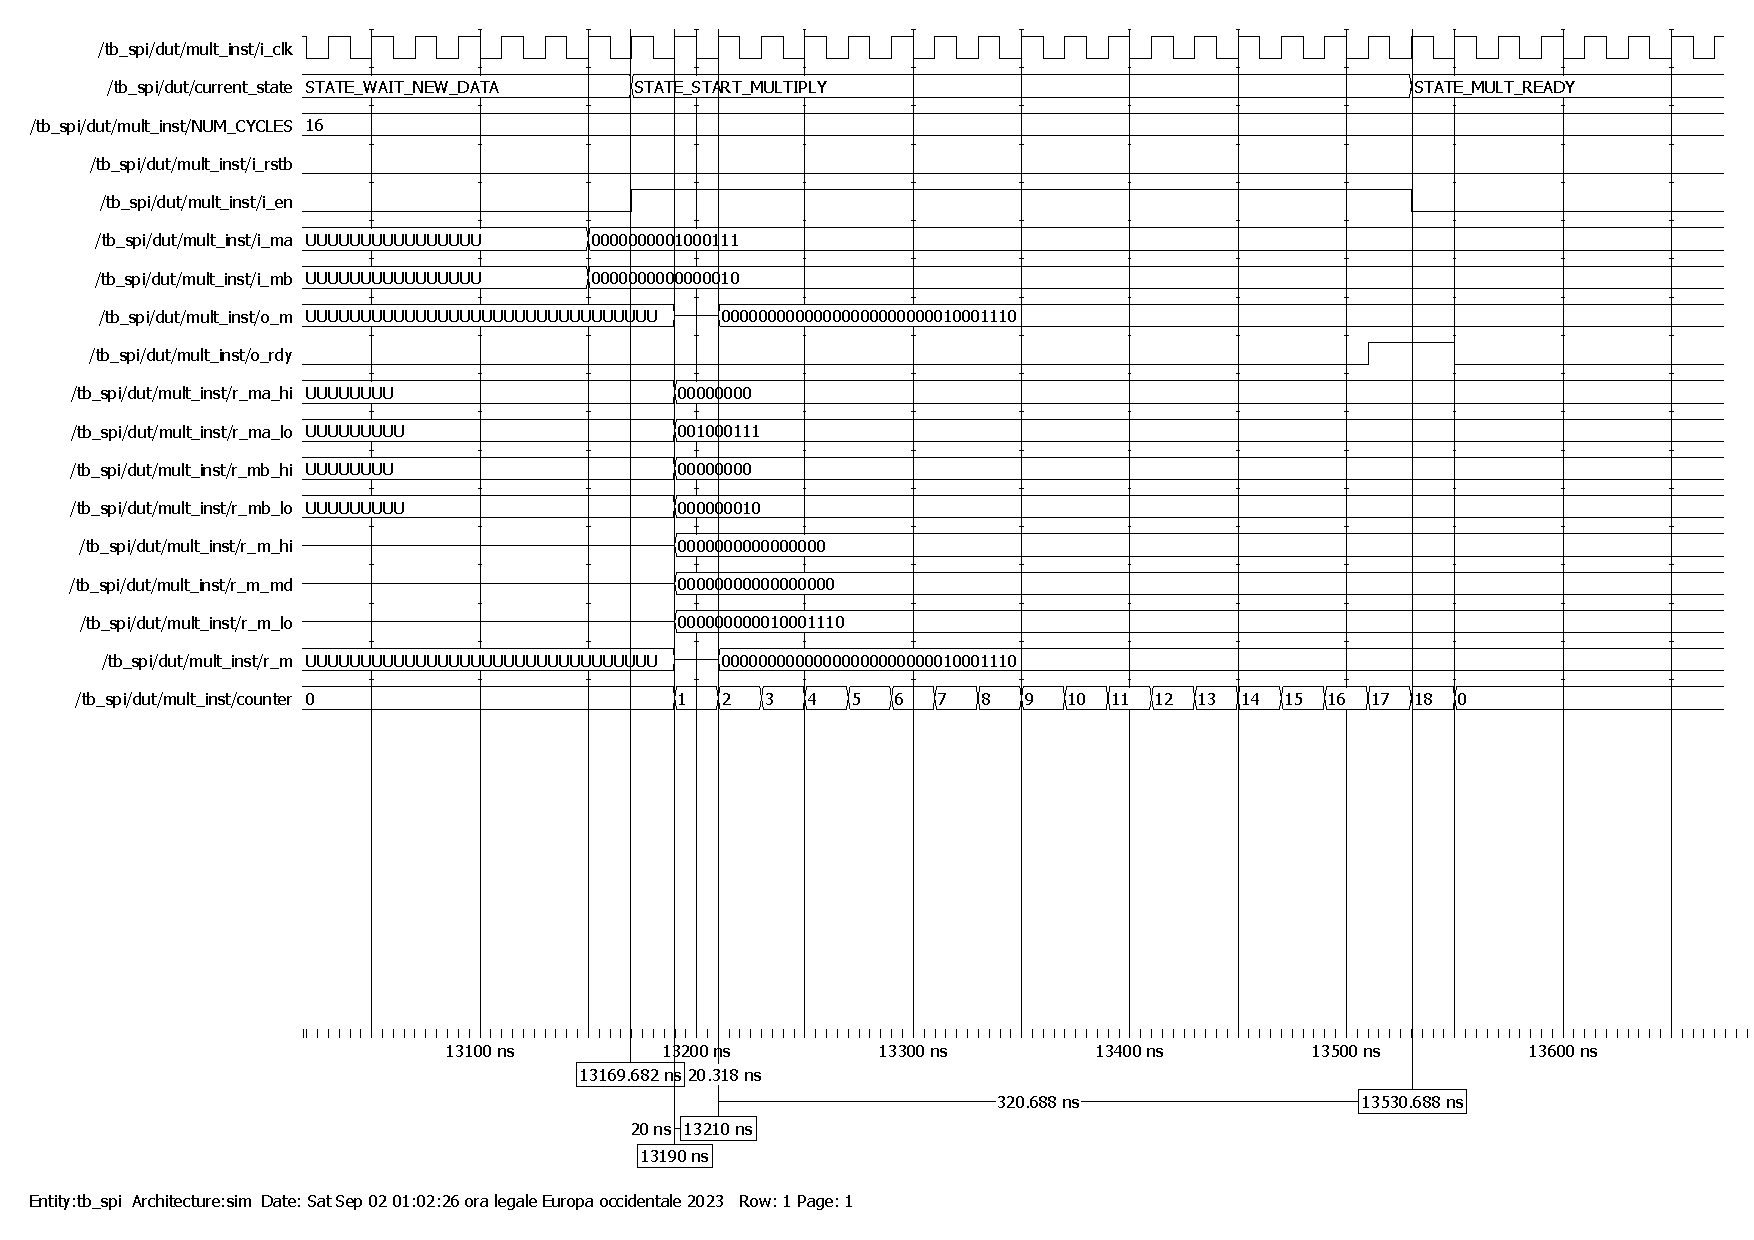
\includegraphics[scale=0.5]{./img/sim_zoom_mult_inside.pdf}
			\caption{Simulazione dell'entity mult\_16x16\_sign\_break ottenuta con Modelsim}
			\label{fig:modelsim_sim_completa2}
		\end{figure}

	\section*{Analisi del funzionamento del sistema con SignalTap Logic Analizer}
	\label{sec:SignalTap}
	\addcontentsline{toc}{section}{Analisi del sistema con SignalTap Logic Analizer}
		In figura \ref{fig:quartus_sim_signaltap} è mostrato l'output dei segnali prodotti dall'FPGA utilizzando l'entity \texttt{basic\_mult}.

		\begin{figure}[H]
			\centering
			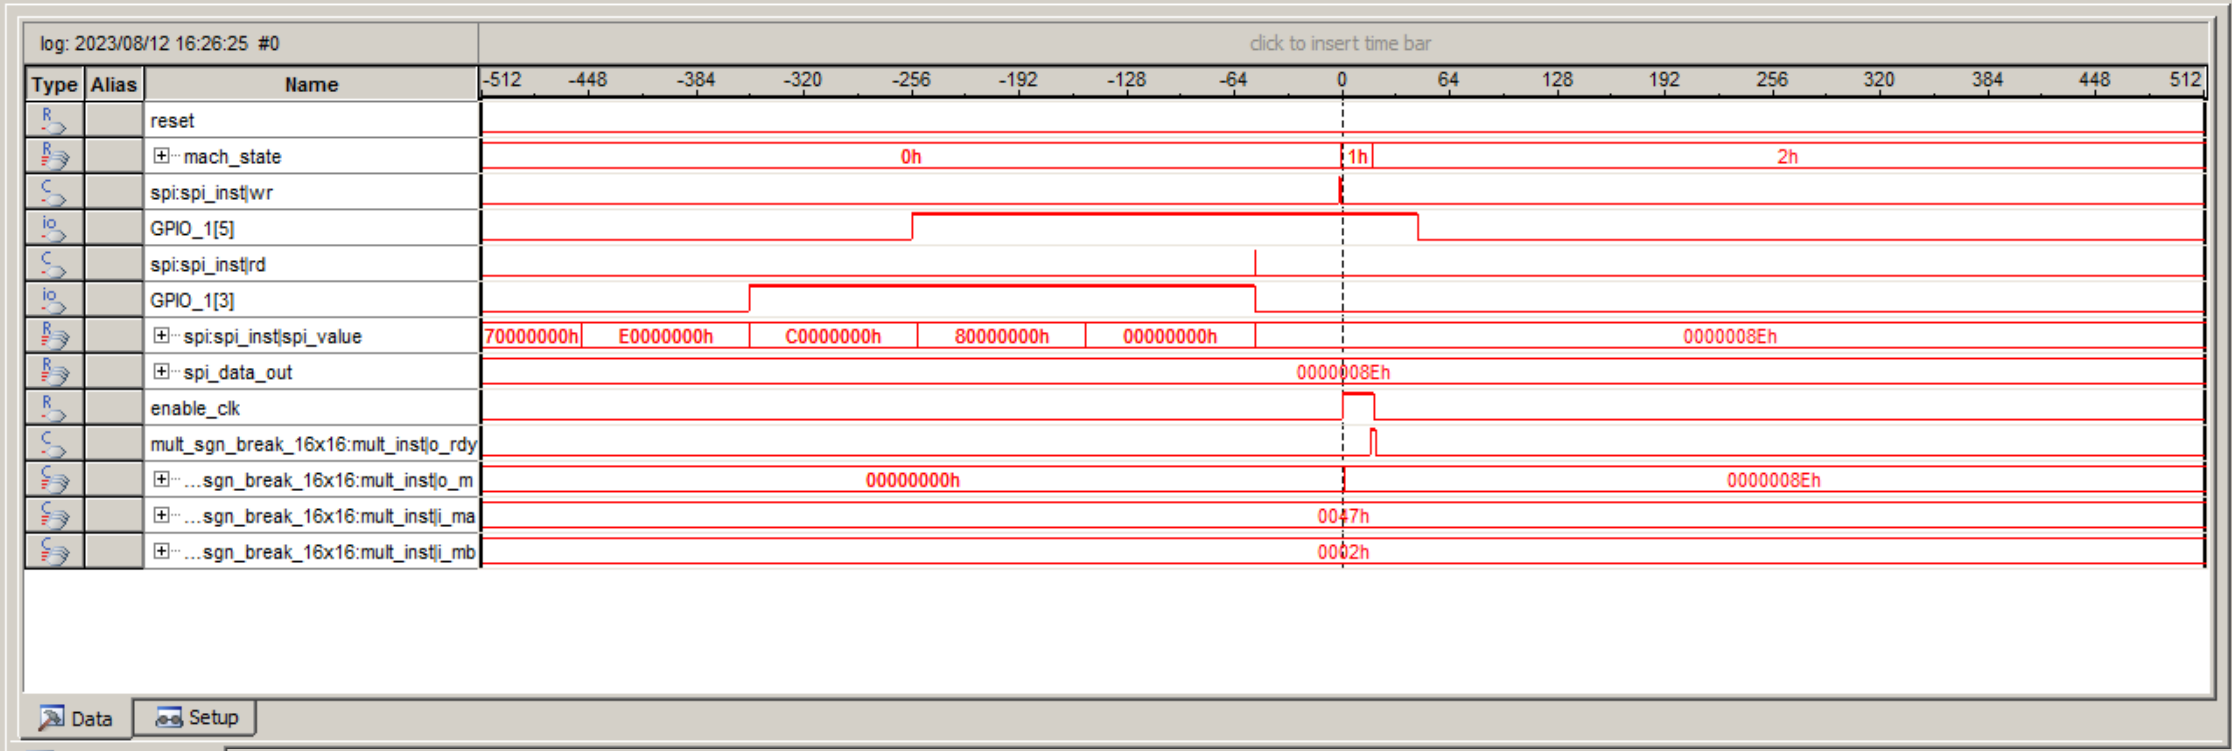
\includegraphics[scale=0.4]{./img/signaltap_multiply_empty.png}
			\caption{Simulazione dell'entity basic\_mult ottenuta con SignalTap Logic Analyzer}
			\label{fig:quartus_sim_signaltap}
		\end{figure}

		In particolare, il trigger per la visualizzazione è stato impostato sul fronte di salita del segnale \texttt{enable\_clk}.
		
		È importante evidenziare anche il cambiamento degli stati del segnale \texttt{mach\_state} e che il risultato ottenuto rispecchi perfettamente la simulazione ottenuta nella sezione \textit{Studio comportamentale}.

		In figura \ref*{fig:quartus_sim_signaltap2} viene riportato il dettaglio della fase di moltiplicazione proponendo i segnali prodotti dall'entity \texttt{mul\_sgn\_break\_16x16}.

		\begin{figure}[H]
			\centering
			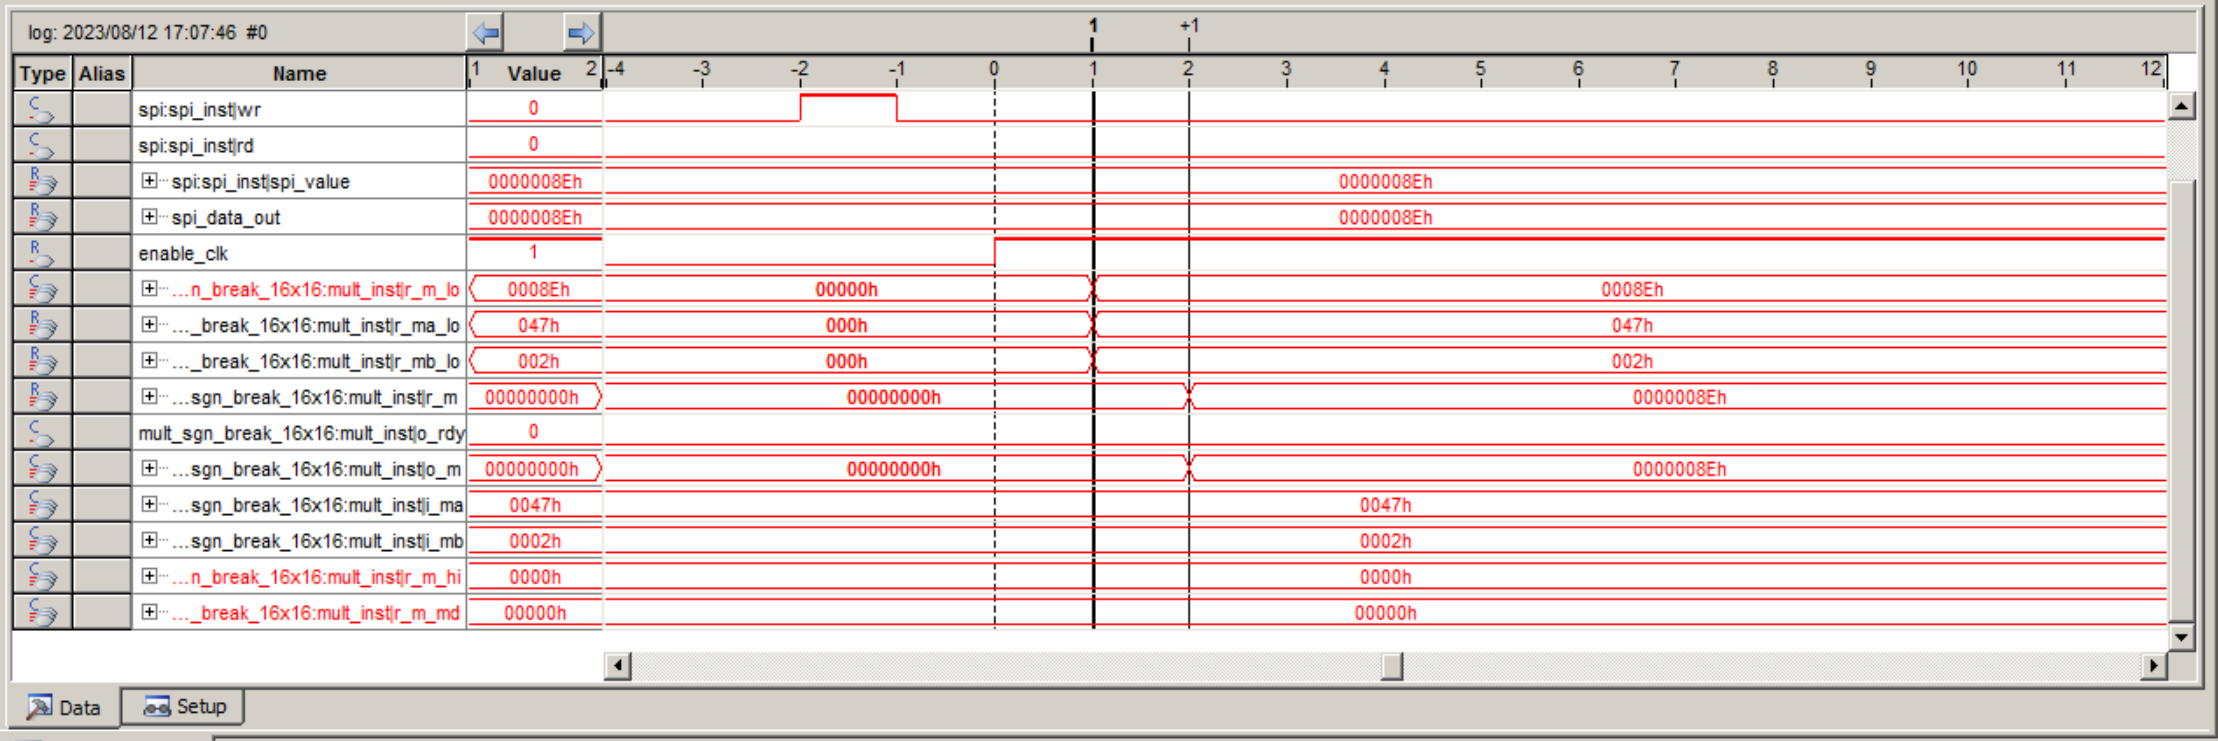
\includegraphics[scale=0.4]{./img/signaltap_multiply_step_by_step.png}
			\caption{Simulazione dell'entity mul\_sgn\_break\_16x16 ottenuta con SignalTap Logic Analyzer}
			\label{fig:quartus_sim_signaltap2}
		\end{figure}

		Anche in questo caso i risultati ottenuti sono in accordo con i risultati proposti dalla simulazione.

\chapter*{Conclusioni}
\label{ch:conclusioni}
\addcontentsline{toc}{chapter}{Conclusioni}
	
	Visti i risultati ottenuti, il sistema rispetta le specifiche di progetto e riesce a produrre il risultato voluto. Sicuramente è un sistema imperfetto che necessita di qualche accorgimento per essere ottimizzato nel tempismo di produzione del dato. Questo potrebbe essere ottenuto utilizzando meglio i l'analisi dei segnali in gioco, in particolare il \texttt{feed\_me} dell'entity SPI come analizzato in precedenza. 

	È sicuramente possibile migliorare l'aspetto implementativo del sistema. Il listato \ref{lst:tb_spi.vhd} presenta alcuni problemi di astrazione che si riscontrano anche in figura \ref{fig:rtl_quartus}. La divisione tra top level e livelli inferiori non è netta come dovrebbe essere da teoria.

	Inoltre, lo script python prodotto per la visualizzazione del dato presenta alcune imperfezioni di lettura, ma non essendo l'obiettivo di questo progetto non è stato perfezionato.


\listoffigures
\listoftables
\lstlistoflistings

\end{document}